%\documentclass[conference]{IEEEtran}
\documentclass[compsoc, conference, letterpaper, 10pt, times]{IEEEtran}
\usepackage{cite}


\usepackage{amsmath}
\usepackage[T1]{fontenc}
\usepackage{ae, aecompl}
\usepackage{color}
\usepackage{booktabs}
\usepackage{paralist}
\usepackage{graphicx}
\usepackage{amsfonts}
\usepackage{times}

\usepackage{float}
%\DeclareCaptionType{copyrightbox}
\usepackage[hyphens]{url}
\usepackage{enumerate}
\usepackage{algorithmicx}
\usepackage{algpseudocode}
\usepackage{algorithm}


\usepackage[caption=false,font=footnotesize]{subfig}
\usepackage{url}

% \usepackage{subcaption}
\usepackage{caption}
\captionsetup[table]{skip=10pt}

\usepackage{multirow}
\usepackage{tikz}

\newcommand{\nn}{\nonumber}
\newcommand{\set}[1]{\mathcal{#1}}        			% Set
\newcommand{\rv}[1]{\boldsymbol{#1}}    			% Random variable
\renewcommand{\vec}[1]{\boldsymbol{\mathrm{#1}}} 	% Vector or Matrix
\newcommand{\event}[1]{\langle #1 \rangle}      	% Event
\newcommand{\arthur}[1]{\textcolor{blue}{Arthur: #1}}
\newcommand{\fixit}[1]{\textcolor{red}{#1}}
\newcommand{\etal}{\emph{et~al.}}

%\usepackage{authblk}


\renewcommand{\itemize}{\compactitem}
 \renewcommand{\enumerate}{\compactenum}

  % Defining dash lines
  \newcommand\solidthinrule[1][.5cm]{\rule[0.5ex]{#1}{.4pt}}
  \newcommand\solidthickrule[1][.5cm]{\rule[0.5ex]{#1}{1.5pt}}
  \newcommand\dashedthinrule{\mbox{%
    \solidthinrule[1mm]\hspace{1mm}\solidthinrule[1mm]\hspace{1mm}\solidthinrule[1mm]}}
  \newcommand\dashedthickrule{\mbox{%
    \solidthickrule[1mm]\hspace{1mm}\solidthickrule[1mm]\hspace{1mm}\solidthickrule[1mm]}}
  \definecolor{darkgreen}{rgb}{0, 0.8, 0}

% Defining checkmark
\def\checkmark{\tikz\fill[scale=0.4](0,.35) -- (.25,0) -- (1,.7) -- (.25,.15) -- cycle;}

\newenvironment{mymathbox}
{\par\smallskip\centering\begin{lrbox}{0}%
\begin{minipage}[c]{0.8\textwidth}}
{\end{minipage}\end{lrbox}%
\framebox[0.9\textwidth]{\usebox{0}}%
\par\medskip
\ignorespacesafterend}

% correct bad hyphenation here
\hyphenation{op-tical net-works semi-conduc-tor}

\begin{document}
\title{Quantifying Web Adblocker Privacy}

\author{
    \IEEEauthorblockN{Arthur Gervais\IEEEauthorrefmark{1}, Alexandros Filios\IEEEauthorrefmark{1}, Vincent Lenders\IEEEauthorrefmark{2}, Srdjan \v{C}apkun\IEEEauthorrefmark{1}}
    \IEEEauthorblockA{\IEEEauthorrefmark{1}ETH Zurich, Switzerland
    \\\{1, 2, 4\}@inf.ethz.ch}
    \IEEEauthorblockA{\IEEEauthorrefmark{2}Armasuisse, Switzerland
    \\\{3\}@armasuisse.ch}
}

\maketitle

\begin{abstract}

Web advertisements, an integral part of today's web browsing experience, financially support countless websites. Meaningful advertisements, however, require behavioral targeting, user tracking and profile fingerprinting that raise serious privacy concerns. To counter privacy issues and enhance usability, adblockers emerged as a popular way to filter web requests that do not serve the website's main content. Despite their popularity, little work has focused on quantifying the privacy provisions of adblockers.

In this paper, we develop a quantitative approach to objectively compare the privacy of adblockers. We propose a model based on a set of privacy metrics that captures not only the technical web architecture, but also the underlying corporate institutions of the problem across time and geography.

We investigate experimentally the effect of various combinations of ad-blocking software and browser settings on 1000 Web sites. Our results highlight a significant difference among adblockers in terms of filtering performance, in particular affected by the applied configurations. Besides the ability to judge the filtering capabilities of existing adblockers and their particular configurations, our work provides a general framework to evaluate new adblocker proposals.

\end{abstract}

\section{Introduction} \label{sec:introduction}




Online advertising provides a viable way to support online businesses that offer content free of charge to their users, such as news, blogs and social networks. To achieve targeted and hence more effective advertising however, advertisers and tracking companies record user browsing behavior, e.g. pages viewed, searches conducted, products purchased~\cite{mayer,barford, krishnamurthy_privacy_diffusion, soltani, Gill13}. Such techniques are known as \textit{online profiling} and have raised significant privacy concerns because online user profiles can be used to infer private sensitive information and user interests~\cite{castelluccia, mikians, datta, libert2015exposing}.

\emph{Adblockers} aim to improve the user experience and privacy by eliminating undesired advertising content, as well as preventing the leakage of sensitive user information towards third-party servers. The most well-known adblocker solutions are browser extensions such as \emph{Ghostery} or \emph{Adblock Plus} which suppress unnecessary requests to third-party advertisements and tracking servers, thereby limiting the risk of data leakage towards these servers. Recently, users' privacy concerns and awareness about online profiling and tracking practices have strongly increased, leading to a proliferation of adblocker browser extensions in the wild. According to Mozilla and Google usage statistics~\cite{Mozilla_statistics,Google_statistics}, already more than thirty million surfers are actively using a browser with the Adblock Plus extension enabled. In a recent measurement  study~\cite{pujol}, researchers show that 22\% of the most active users are using the Adblock Plus adblocker while surfing the Web.

Despite the popularity of adblocking tools, surprisingly little research has been performed to  understand how well adblocking actually improves the privacy of its users. While the methods employed in advertisement and tracking and their privacy implications have been well researched in the literature~\cite{krishnamurthy_measuring_privacy_loss, leon, englehardt,nikiforakis}, the protection that adblockers offer, has not been investigated that much in the literature. Works such as~\cite{pujol, butkiewicz, ruffel2015, kontaxis} analyze ablockers's performance, however the impact of user privacy is not in the main scope of these studies, as they focus on the effectiveness of the adblocker's implementations and the usage in the wild.
Understanding how adblockers affect user privacy is fundamental to their use, because it not only provides feedback to the users, but also helps at correctly using and configuring those systems. Adblockers rely on complex filter configurations in the form of blacklisted URLs and regular expressions, and as we show in this paper, existing adblockers are not necessarily configured by default to provide the best privacy protection to their users.


%but tradeoff privacy for the support of content providers which rely on "non-intrusive" advertisements for their main stream of revenue.










%Libert~\cite{libert2015exposing} for example has shown that nearly 9 in 10 websites leak user data to parties likely unknown to the user.


%Juniper Research estimates in a recent study that digital publishers are going to lose over 27 billion dollars by 2020 due to the use of ad blocking services~\cite{Juniper_study}. Therefore, some players

%while popular, the protection is unclear in terms of privacy
% ads and tracking companies are paying to be whitelisted
% maintainers of blacklists lag
% The effect of page load time and user experience has been analyzed in [], but there is no study on the effect of these tool on user privacy.



%Because of their privacy-critical character, related work already attempted the evaluation and comparison of the privacy blocking performance of web browser based adblockers~\cite{pujol, ruffel2015, mayer, englehardt}. Existing literature has often employed the number of blacklisted domains, cookies or HTTP requests as a privacy index~\cite{butkiewicz, pujol, kontaxis}. We observe that these metrics do not take into account legal entities (i.e., the companies behind third party domains) nor the temporal aspect of the adblocker filtering performance. Furthermore, although the widespread usage of mobile devices has markedly changed the landscape of web browsing over the last years, little focus has been laid on the web privacy for mobile devices.

Our goal in this work is to quantify the privacy that web adblockers provide. We address this problem by developing a quantitative model to compare adblocker filtering performance across various privacy dimensions. Our model includes simple count metrics to third-parties, but also considers more advanced metrics on the level of organizations (legal entities) and countries as well as their relationships. In order to also understand the temporal dynamics of the system, we further incorporate temporal metrics to track the filtering performance over time.

%While previous works have analyzed the effect of adblockers on reducing the number of advertisements and improving page load performance~\cite{}, to the best of knowledge, this paper is the first to focus on quantifying the privacy benefits of adblockers.
%To this end, we define a set of privacy metrics capable of capturing the adblocker's filtering performance and user's privacy implications. % explain the different dimensions: time, entity, countries, etc

We have developed a testbed system which allows us to repetitively browse the same Web sites in a systematic way and classify the number of HTTP requests that go to first and third parties without any classification errors.
We evaluate 12 different browser profile configurations in our testbed, capturing different adblocker instances and combinations of desktop/mobile user client agents. During three weeks, we repetitively surfed Alexa's top 500 global sites and 500 randomly selected sites and analyzed how different configurations influence these privacy metrics.

%We moreover study the adblocker filtering performance over a timespan of three weeks in order to assess the temporal stability of their blocking capabilities. Lastly we capture the legal corporations as well as the geographical locations behind the third parties.

Our results show that the usage of adblockers provides a significant improvement in terms of user privacy.
However, the degree of protection is highly depending on the configuration. For example, by default Ghostery does not block any third-party requests and Adblock Plus still allows a significant amount of requests to third parties. These results are consistent for the desktop and the mobile user agents. When increasing the level of protection in Ghostery and Adblock Plus however, these tools manage to effectively suppress requests to third-parties and thus improve the privacy. Except for Google Inc. which still receives around 50 \% of third-party requests because it hosts relevant content not related to advertisement and tracking, the amount of third-party requests towards the other top ten companies in our experiments is only 2.6 \% of the total amount that would result when surfing without an adblocker.



%More specifically, the Ghostery adblocker consistently performs better than AdblockPlus when both adblockers are set to the maximum-protection level. In the default settings however, Ghostery does not block third-party. Our results show that the usage of the \textit{do not track} header prevents the loading of a few third parties. We do not observe a significant difference between mobile and desktop clients with respect to the number of loaded third parties.

Our contributions in this paper can be summarized as follows:
 \begin{itemize}
 \item We provide a quantitative methodology to objectively compare the filtering performance of web adblockers.
 \item We capture the temporal evolution of adblocker filtering performances and study the differences between mobile and desktop devices, as well as the impact of the \emph{do not track} header. Our methodology further allows to measure the influence of other parameters (e.g. third-party cookies) on adblocker filtering performance.
 \item Beyond the domain of the third parties, our model takes into account the underlying legal entities, their corresponding geographical locations as well as their relationships.
% \item Our measurement methodology allows us to capture with 100\% accuracy the first and third parties during our evaluation.
 \item Using our model, we quantify the privacy of 12 different adblocker browser profile configurations over 1000 different Web sites for repetitive daily measurements over the duration of three weeks and discuss the implications in terms of user protection.
\end{itemize}

The remainder of the paper is organized as follows. In Section~\ref{sec:background} we illustrate the objective and functionality of adblockers, while in Section~\ref{sec:privacy_metrics} we outline our privacy metrics. Section~\ref{sec:evaluation} discusses the experimental setup and the results. Section~\ref{sec:related_work} presents the related work and Section~\ref{sec:conclusions} summarizes our work.

\section{Web Tracking and Adblockers Background}
\label{sec:background}
%Web Privacy is an often-mentioned and thoroughly-analyzed field of study.
This section provides relevant background on third-party tracking  in the web and how adblocker browser extensions aim at improving user experience and privacy.

\subsection{Third-party Tracking}

When visiting an HTTP-based website on a domain (commonly referred to as first party), the web browser sends an HTTP request to the first-party server that hosts the website and loads the content of the first-party domain. The HTML code of the first party is then able to trigger (without the awareness of the user) further HTTP requests to remote servers (commonly referred to as third parties) in order to load further resources that they host. External resources vary in their format and are applied with different objectives, such as the inclusion of external libraries ---e.g. jQuery--- that are indispensable for the functionality of the website itself. Further reasons include the promotion of advertising content that can be externally loaded and placed at a pre-allocated space on the website.

This third-party content loading mechanism clearly facilitates the development and deployment of dynamic websites because it allows to use different content providers to load resources that do not need to be served from the first party. However, as shown in previous works~\cite{mayer,barford, krishnamurthy_privacy_diffusion, soltani}, HTTP requests to third-parties lead to severe privacy implications because third parties can follow the activity of the users and reveal the pages they are looking at while surfing the web. For example, it has been shown in ~\cite{Gill13} that dominant players in the market such as Google Inc. are embedded as third-parties in so many web sites that they can follow 80 \% percent of all web activities. Since the web page content and thus user interests can be inferred by the uploaded requests to the third parties, personal profiles of users can easily be derived and potentially used to discriminate people or spy on their interests and habits without getting noticed by the users.

\subsection{Adblocker browser extensions}



To address the aforementioned implications and challenges, numerous software and hardware-based solutions --- commonly referred to as \textit{adblockers} --- have been proposed in order to remove or alter the advertising and third party content in a web page. Although there exist multiple ad-blocking methods (e.g. DNS sinkholing, proxies run by internet providers (externally) or by an application on the same client machine, special hardware) we focus in this work on one of the most popular solutions: browser extensions, such as \textit{Ghostery} and \textit{AdblockPlus}.
%TODO: Maybe add more examples of adblockers, since we didn't introduce our model yet and we're generally speaking

Adblocker browser extensions use one or more lists that describe the content that is to be allowed (whitelists) or blocked (blacklists) and update those on a regular basis. There are two principal methods how adblockers apply these lists to remove ads/third parties from a web page: One is filtering the resource according to the result of an URL-pattern matching, before this resource is loaded by the web browser. The second consists in hiding loaded content with the use of CSS rules (\textit{element hiding}) within the HTML content. In terms of privacy, filtering the resources before they are requested by the browser is the only effective method because these requests are the ones revealing the activity of the users.

Adblocker browser extensions are very popular by users today and their popularity is continuously on the rise~\cite{Mozilla_statistics,Google_statistics,pujol}. However, content providers and advertisers see this trend as a risk to their own business models because they regard the application of theses tools as a way for the comsumers to evade "paying for the content". Juniper Research estimates that digital publishers are going to lose over 27 billion dollars by 2020 due to the use of ad blocking services~\cite{Juniper_study}. There is therefore high pressure by these industries on the developers of adblockers to not blacklist their services. For example, Adblock Plus has introduced in 2011 the concept of "non-intrusive advertising", which basically allows third-party advertisements for ads which do not \emph{disrupt the user's natural reading flow}~\cite{acceptable_ads}. However, these practices raise concern in terms of privacy because non-intrusive advertisement services may well perform intensive tracking without falling in this category.  We therefore argue that it is important to quantify independently the privacy of these tools as we do in this work.






%Although third parties clearly improve the web's functionality, they come with a series of implications that have been subject of controversy:
%\begin{itemize}
% \item security threats, e.g. malware attacks~\cite{cisco_annual_security_report}
% \item privacy risks, e.g. fingerprinting and tracking~\cite{englehardt, krishnamurthy_privacy_diffusion, nikiforakis, soltani}
% \item user distraction through advertisement, e.g. reader distraction~\cite{beymerl}, limited retention of website content~\cite{mccoy}
% \item performance and data overhead, e.g. page-loading slowdown~\cite{krishnamurthy}
%\end{itemize}



\section{Privacy Model and Metrics}
\label{sec:privacy_metrics}
In this section, we introduce our privacy model and the  metrics we use in order to quantify the privacy provisions of adblockers.

\subsection{Threat definition}
A key issue for a threat model in adblocking is to define which third-parties should be considered as a privacy threat to users. In this work, we consider all third-parties as potential threats irrespective of the type and content of the queries towards these third parties. This approach may arguably seem conservative, but it is practically impossible to exclude for sure any third-party from performing tracking and/or profiling given the multitude of possible mechanisms that are available and continuously invented for fingerprinting and tracking user behavior in the web.

In our notion, the privacy objective of the abblocker is therefore to reduce as many requests as possible towards third parties. Notice here the difference of our threat model definition to the slightly different objective that adblockers such as Adblock Plus have. By default, Adblock Plus aims at improving user satisfaction by minimizing the display of intrusive advertisements which annoy the users while third-party requests to non-disturbing advertisements and tracking services for commercial purposes are considered to be acceptable~\cite{acceptable_ads}.


\subsection{User tracking model}
\label{sec:graph_definition}
We model the tracking of a user $U$ through third parties as undirected graph $G=(E,V)$, where $E$ are edges, and $V$ vertices. A vertex $V_S$ represents a web domain and is connected to another vertex $V_T$ through an edge $E$, if and only if at least one request has been sent from $V_S$ to $V_T$. In that case, $V_S$ is the \textit{source} of the request and $V_T$ the \textit{target} of the request.

In the following, we use the term \textit{third-party request} (TPR) to denote the requests that are sent to a target domain $T$ that differs from the source domain $S$ and corresponds to a graph edge $E$ between the nodes $V_S$ and $V_T$. On the contrary, the requests whose source and target coincide are designated as \textit{first-party requests} (FPR) and are not taken into consideration for the construction of $G$, since no information leaks to third parties and hence they do not bring about further risks for user's privacy\footnote{Arguably, users also leak private information to first party domains when they visit and interact with those sites, however, since users are visiting these first parties deliberately, the privacy risks are known to the users and controllable without an adblocker.}. The source and the target domain are referred to as \textit{first-party domain} (FPD) and \textit{third-party domain} (TPD) and correspond to FPD and TPD graph nodes, $V_S$ and $V_T$, respectively.

Compared to previous works on third-party traffic characterization~\cite{butkiewicz,englehardt}, we augment \emph{G} by incorporating the ownership of third party domains to their corresponding legal entities, i.e. the organizations who own the different TPDs. Two TPD, belong to the same legal entity if they are registered to the same organization (e.g., doubleclick.net and google-analytics.com both belong to Google Inc.) and are thus combined into one vertex, resulting in a hierarchical graph (cf. Figure~\ref{fig:graph}). Considering the information flow of third-party requests towards legal entities is particularly important for the scope of privacy because legal entities which own multiple domains can fuse the information they collect from their different domains in order to increase their tracking and profiling coverage, thus resulting in a higher privacy threat to the users.

Finally, we further attribute each legal entity to a geographical location (the country where the headquarter of the legal entity is situated) in order to model which countries govern the regulations over which legal entities. This geographical perspective is also of special importance to privacy, because most data privacy laws are specific to local laws of the countries, thus affecting the regulations that apply to the user data that is collected by the legal entities.

\begin{figure}[tb!]
  \centering
  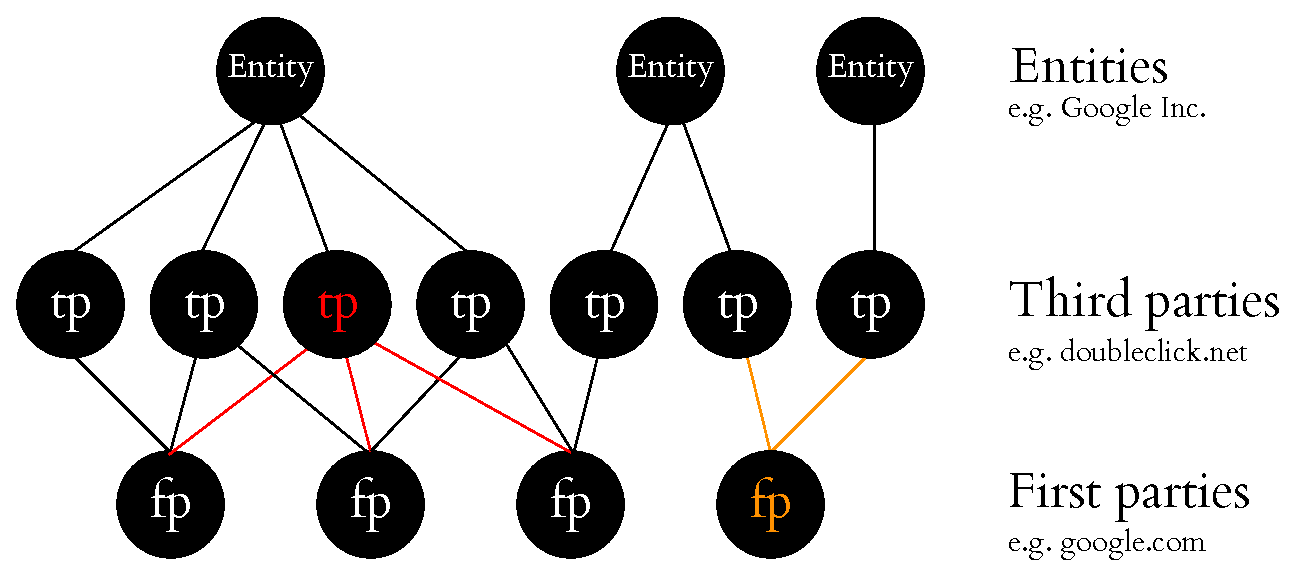
\includegraphics[width=0.45\textwidth]{figures/graph.eps}
  \caption{Graphical representation of our user tracking model. The colored third-party domain (TPD) has a node degree of~3, the colored first-party domain (FPD) has a node degree of~2. The colored third-party entity (TPE) spans all its child TPD nodes and hence has a degree of~3.}
  \label{fig:graph}
\end{figure}



\subsection{Privacy Metrics}

Given the graph representation \emph{G} of our user tracking model, we evaluate the respective privacy provisions based on the following metrics.

%In the following section we elaborate our privacy metrics to quantify the privacy provisions of web adblocker. We categorize the privacy metrcis in \emph{(i)} first order relationships, \emph{(ii)} graph metrics and \emph{(iii)} the temporal change.

%\subsubsection{First Order Relationships}
%We outline in the following two primary privacy metrics that are captured via the first order relationship between FPDs and TPDs.

\subsubsection{Degree of First Party Domain}
The degree of a FPD node of graph $G$ refers to the number of TPDs that it has sent at least one third-party request to when loading the web page from the FPD. That is, the more edges a FPD node has --- or, equivalently, the more third parties loaded by a first-party --- the more third parties are able to track the web-browsing history of a user. The FPD node degree is a metric that is commonly used to evaluate the adblocker's performance~\cite{ruffel2015}. However, it is alone not a sufficient metric to capture the impact on user privacy, as it does not represent the structure behind the relationships between FPD and TPD. The following metrics therefore aim at capturing these relationships.

\subsubsection{Degree of Third Party Domain}
The degree of a TPD node can be directly translated to the number of first-party websites that a particular third party exchanges information with and potentially tracks. Clearly, the more often a third party is accessed over the user's series of websites $S_U$, the less privacy the user experiences from this particular third party. To exemplify this statement, let's assume that a third party is requested by only one of the first-party websites $S_U$ visited by $U$. This third party will in this case learn that the user has accessed the respective first party, but has a limited view of their browsing behavior. If the third party, however, is requested by over 80\% of the user's visited websites, $S_U$, the third party will likely be able to recover up to 80\% of the web behavior of $U$.

%We capture this privacy notion by assessing the degree of the TPD nodes in the graph $G$ so as to evaluate the improvement that the ad-blocking software can achieve.

\subsubsection{Degree of Legal Entity}
\label{sec:legal_entity}
Instead of focusing on domain degrees, the degree of a legal entity reflects the number of third-party domains that belong to a legal entity. Third-party domains such as \url{doubleclick.net} and \url{google.com} for example are both owned by the same entity Google Inc. Their collusion therefore seems more likely, and affects the privacy of a web user $U$ more significantly, than if both were belonging to two different legal entities. By incorporating the legal relation among third party domains, we therefore capture a more realistic privacy leakage through user web surf activity.

\subsubsection{Geographical location}
After having mapped the TPD's to legal entities, we further assign a geographical location to the TPD. This allows our model to capture the geographical distribution of the TPDs and thus infer which geographical countries have for instance the most TPD. The geographical location of a legal entity is defined by the country in which its headquarter resides. Alternatively, we could consider the particular location of the servers as derived from the IP address, but content retrieved from web services is often hosted on distributed caches and content distribution networks and hence the server IP address does not necessarily reflect the country to which the user data is finally sent to. By choosing the headquarter's location, we thus aim at modelling the country in which the privacy laws and regulations will apply to the user data as collected by the third-party.


\subsubsection{Graph Density}
In addition to the degree metrics outlined above, we consider a metric based on the graph density of $G$. Since an edge on the graph $G$ represents a partial tracking relationship between a third and a first party, we expect that the denser the graph $G$, the more information can be retrieved by third parties/can leak to third parties with respect to the browsing behavior of the user. We observe that the more dense $G$ is, the more third parties are likely able to track the user $U$. The graph density therefore allows to reason about the possible privacy improvements by the respective ad-blocking software. We rely on a common definition of the graph density as:
\begin{equation}
\label{eq:density}
D = \frac{2 |E|}{|V|(|V|-1)}
\end{equation}

Note however that we cannot achieve the maximum density of 1, because the first parties in $G$ are not directly connected (cf. definition in Section~\ref{sec:graph_definition}).

\section{Evaluation Methodology}

In order to compare the privacy of different adblockers, as well as the influence of different browser settings on their adblocking efficiency, we create different browsing configurations without adblockers, with the Ghostery, and with the Adblock Plus browser extenstions installed in the Firefox browser.

\subsection{Considered Browser Profiles}

\begin{table*}
\centering
\begin{tabular}{|c|c c c c|}
\hline
\multirow{2}{*}{Protection Level} & \multicolumn{4}{|c|}{Lists} \\
& AdServers & EasyList & EasyListChina & EasyPrivacy \\
\hline
Default & & \checkmark & & \\
Maximal & \checkmark & \checkmark & \checkmark & \checkmark \\
\hline
\end{tabular}
\caption{AdblockPlus blacklist combination for default and maximal protection level. Ghostery's default and maximal protection correspond to the selection of none and all tracker categories, respectively.}
\label{table:blacklists}
\end{table*}


All our experiments are performed on "Linux (Release: Ubuntu 14.04.4 LTS, Version: 4.2.0-35-generic GNU/Linux)" with the version 45.0.1 of the Firefox browser. For Ghostery, we use the browser plugin version 6.1.0 and for Adblock Plus the plugin version 2.7.2.
The different protection levels, \textit{Default} or \textit{MaxProtection}, for the two adblockers \textit{AdblockPlus} and \textit{Ghostery} respectively, are achieved through the use of a different combination of blacklists. AdblockPlus and Ghostery store their respective blacklists in the form of URL and CSS regular expressions. The blocking options of AdblockPlus are set through the direct inclusion of blacklists to be applied, while  Ghostery's blacklist configuration consists in the selection among a multitude of tracker categories to be blocked. An overview of these configurations is presented in Table~\ref{table:blacklists}.



%We argue, that \emph{(i)} regular expressions cannot be compared easily and \emph{(ii)} that blacklists alone are insufficient in order to judge about the blocking capability of an adblocker because the regular expressions have to be applied to a dataset of URLs. Intuitively, each blacklist entry (regular expression) does not contribute equally to the blocking performance of the adblocker. That is because some regular expressions \emph{hit} more often than others, depending on the accessed URL set. The addition (or deletion) of regular expressions to the blacklists therefore does not provide an objective measure to judge about the improvement of a blacklist.



%. Ghostery's block policy is configured through the selection of trackers to be blocked from a pre-defined list provided by the plugin. By default no tracker is blocked and in maximum-protection settings, all trackers are blocked.

%We use Adblock Plus version ???. Adblock Plus' policy is defined by the activation of publicly available blacklists. By default, ``EasyList'' is activated, whilst in maximum-protection settings, the activated blacklists are ``EasyList'', ``EasyList China'', ``EasyPrivacy'' and ``Peter Lowe's List''.

Modern web browsers such as Firefox further allow to set the \emph{do not track} HTTP header option, to express their personal preference regarding tracking to each server they request content from, thereby allowing recipients of that preference to adjust tracking behavior, accordingly~\cite{dnt}. It remains the sole responsibility of the web server to respect the request of its clients. Almost 10\% of the Firefox users have enabled this option on their desktop browsers in 2014~\cite{dnt_state_firefox}. In order to evaluate to which extend the DNT header has an influence on our proposed metrics we as well include the DNT option in our evaluation.

The usage of mobile devices for web browsing has recently witnessed a steady growth~\cite{mobile_usage}. As a consequence, an ever increasing number of websites has been adapting to the demands of the mobile user agents. Because of the dimensions and the reduced-bandwidth requirements of the mobile devices, the structure and content of the web pages has to be adjusted accordingly and the advertising content could not remain unaffected by these limitations. To investigate the effects of user agents from a privacy-related perspective, we consider this parameter in the design of the experimental evaluation and evaluate several mobile-device instances by setting the HTTP header \textit{User-Agent} accordingly.

Based on above mentioned criteria, we create 12 browser profiles, $U$ as described in Table~\ref{table:browser_profiles}. Each configuration is defined as a combination of the following parameters :
\begin{itemize}
 \item Adblocker: No adblocker, Ghostery, or Adblock Plus
 \item Block policy: maximum or default protection
 \item User agent: mobile or desktop
 \item Do Not Track (DNT): header enabled or disabled
\end{itemize}
Throughout the remaining of the paper, we use the following conventions for each browser profile $U$ (cf. Table~\ref{table:browser_profiles}):
\begin{itemize}
 \item The \textit{color} denotes the adblocker installed.
 \item The \textit{line width} indicates the protection degree ---i.e.\ default, maximum protection or DNT header.
 \item Profiles with Mobile User Agent are plotted in \textit{dashed lines}.
\end{itemize}
%The data collected for browser profile $U$ on a specific date correspond to a different graph $G$. The plot legends corresponding to each browser profile $U$ are described in Table~\ref{table:browser_profiles}.

  \begin{table*}
  \centering
  \begin{tabular}{|c|c c c c c|}
  \hline
  Browser Profile & Adblocker & Block Policy & DNT & User Agent & Legend \\
  \hline
  Ghostery\_Default & Ghostery & Default & No & Desktop  & {\color{red}\solidthinrule} \\
  Ghostery\_MaxProtection & Ghostery & Max & No & Desktop & {\color{red}\solidthickrule} \\
  Adblockplus\_Default & AdblockPlus & Default & No & Desktop & {\color{blue}\solidthinrule} \\
  Adblockplus\_MaxProtection & AdblockPlus & Max & No & Desktop & {\color{blue}\solidthickrule} \\
  NoAdblocker & None & - & No & Desktop & {\color{darkgreen}\solidthinrule} \\
  NoAdblocker\_DNT & None & - & Yes & Desktop & {\color{darkgreen}\solidthickrule} \\
  Ghostery\_Default\_MUA & Ghostery & Default & No & Mobile & {\color{red}\dashedthinrule} \\
  Ghostery\_MaxProtection\_MUA & Ghostery & Max & No & Mobile & {\color{red}\dashedthickrule} \\
  Adblockplus\_Default\_MUA & AdblockPlus & Default & No & Mobile & {\color{blue}\dashedthinrule} \\
  Adblockplus\_MaxProtection\_MUA & AdblockPlus & Max & No & Mobile & {\color{blue}\dashedthickrule} \\
  NoAdblocker\_MUA & None & - & No & Mobile & {\color{darkgreen}\dashedthinrule} \\
  NoAdblocker\_DNT\_MUA & None & - & Yes & Mobile & {\color{darkgreen}\dashedthickrule} \\
  \hline
  \end{tabular}
  \caption{Overview of browser profiles examined}
  \label{table:browser_profiles}
  \end{table*}


\subsection{Experimental Setup}

The distinction between FPRs and TPRs is crucial in our attempt to precisely quantify the filtering capability for each browser profile, since they define the exact topology of the derived graph $G$.
Passive classification of HTTP requests into first-party and third party requests is not a trivial task given the complex and dynamic structure of Web pages~\cite{pujol}. For this reason, we rely in this work on an active approach in which we collect our own synthetic web surfing traffic with  automated web surfing agents. To create a realistic and representative dataset, the agents visits Alexa's top 500 web sites (the 500 domains with the highest incoming traffic in the web) and 500 web sites which are sampled uniformly among Alexa's top 1~million most-visited domains. The motivation for including less popular web sites is to avoid the risk of favoring an adblocker optimized to perform best for the most popular web sites, eventually biasing the experimental results. The overall sample set $S$ of 1000 URLs is retrieved once and kept unchanged throughout the evaluation period, so as to de-correlate any variations of the results between different days.

%An appropriate criterion for the evaluation of an adblocker is its filtering performance in the most frequent case. Consequently, it is plausible to test its efficiency for instance on the \textit{500 domains with the highest incoming web traffic}. Considering the top-visited domains, however, would imply the risk of favoring an adblocker optimized to perform better for a certain group of websites, eventually biasing the experimental results. We therefore extend our URL sample set with another \textit{500 uniformly-selected domains} among the top 1 million most-visited domains from the Alexa Traffic Rank. The sample set $S$ of 1000 URLs is stored and kept unchanged throughout the evaluation period, so as to de-correlate any variations of the results between two different days.

Since nowadays most web applications are based on asynchronous calls to fetch data, it is insufficient to wait for the DOM to finish rendering to record all resource requests sent from the website to any first or third parties. To collect the complete data and better evaluate the common user browsing behavior, our agent therefore waits 20 seconds on each website of our sample set $S$ and records any requests sent, before closing and proceeding to the next domain.


We visit the same set of web sites every day during three weeks from 28/04/2016 until 19/05/2016. To decouple the experimental conditions from the influence of any time- or location-related effects ---i.e. variations of the served content, locale-based personalization--- all browser profiles $U$ execute the same crawling routine simultaneously, whilst running on the same machine, thus behind the same IP address, browser and operating system. However, some of the instances are configured to send their requests with a User-Agent HTTP header that corresponds to a mobile device (iPhone with iOS 6\footnote{User Agent: \texttt{Mozilla/5.0 (iPhone; CPU iPhone OS 6\_0 like Mac OS X) AppleWebKit/536.26 (KHTML, like Gecko) Version/6.0 Mobile/10A5376e Safari/8536.25}}), in order to extend our observations for mobile users.

In order to record all HTTP requests, we rely on the \textit{Lightbeam} plugin. However in contrast to~\cite{ruffel2015}, we do not use Lightbeam to determine the source domain that a request is initiated from and to classify it accordingly as a FPR or a TPR because Lightbeam relies on heuristics that are too error-prone for our purpose.
More precisely, the classification of Lightbeam is not always in accordance with our definitions of FPR and TPR, as introduced in Section~\ref{sec:privacy_metrics}. By examining the request logs after a complete crawl cycle and comparing the estimated source to the actual visited domain, two types of false-positive cases (cf. Table~\ref{table:false_positive_examples}) arise in Lightbeam:

\begin{itemize}
\item \textbf{Unrecognized TPRs:} The request is mistakenly considered to be a FPR according to the Lightbeam heuristics, this way ``hiding'' a TPR edge from the graph.
\item \textbf{Misclassified TPRs:} The request is correctly found to be a TPR, but not for the correct FPD node, i.e.\ the one corresponding to the actually crawled domain. The inaccuracy introduced to the graph results from the potential introduction of a bogus FPD node, as well as the false number of TPR edges starting from the correct and the bogus FPD nodes.
\end{itemize}

As results from the experimental evaluation on the data of one full crawl cycle (1000 visited first parties) and 12 different browser profiles, the misclassified and unrecognized TPRs make up for 2.0\%-12.0\% and 4.0\%-11.0\% of the total requests, depending on the respective browser profiles that we define in the following.

\begin{table}
\centering
\footnotesize
\begin{tabular}{|c|c c c|}

\hline
& Visited Domain & Estimated Source & Target \\
\hline
Recognized & wp.pl & wp.pl & facebook.com \\
Misclassified & wp.pl & facebook.com & fbcdn.net \\
Unrecognized & wp.pl & facebook.com & facebook.com \\
\hline
\end{tabular}
\caption{Examples of misclassified and unrecognized TPRs}
\label{table:false_positive_examples}
\end{table}


We thus modify Lightbeam to account for the currently visited first-party as a priori known by the agent which triggers page visits.




%Related work~\cite{ruffel2015} has adopted Lightbeam to capture the TPRs. Nonetheless, Lightbeam does not always know the exact source of each HTTP request sent from our browser. As a consequence, it implements heuristics to determine the source domain that a request is initiated from and afterwards classifies it accordingly as a FPR or a TPR.




\subsection{Classification of Domains to Legal Entities and Locations}
We infer the legal entities' domains and locations by inspecting the WHOIS database. The WHOIS database provides information about the holders of Web domains. For each domain, we look up the legal entity that is registered as holder and the country of the holder's address. Note that only a part of the considered domains ---accounting for about 60\%--- could be assigned to a legal entity and followingly to a country. One reason is that WHOIS does not provide sufficient information for all of the domains loaded. Moreover, our parser that allowed for the automated extraction of the entity information depends on a relatively uniform format of the WHOIS documents and as a result, deviations from this format causes information loss.

\section{Evaluation}
\label{sec:evaluation}
We examine the impact of the configuration parameters on the achieved privacy level using our privacy metrics from Section~\ref{sec:privacy_metrics}.

%\subsubsection{Temporal change}
%The formerly presented metrics only allow us to reason about the privacy provisions of the advertisement blocking software at a given time $t$. The advertisement industry, however, operates dynamically by using e.g., new advertisement techniques and new third party URLs. Within our model we therefore capture the temporal change of the first order relationships (degree of third and first party respectively) and the graph density metric. We do so by evaluating the respective metrics over a time-span and are thus able to judge about the temporal stability of the proposed metrics.

%\paragraph{Blacklist changes}
%In addition to the temporal changes of our metrics, we as well capture when an adblocker updates its blacklist --- we thus observe the update behaviour of the respective adblocker instances, an indicator of how fast the adblocker adapts to the changing advertisement environment.



\subsection{Effectiveness of Adblockers at Suppressing Third-party Requests}
\subsubsection{Baseline without adblocking}

  \begin{figure}
 \centering

 %\subfloat[Scatterplot for the 500 top-ranked sites]{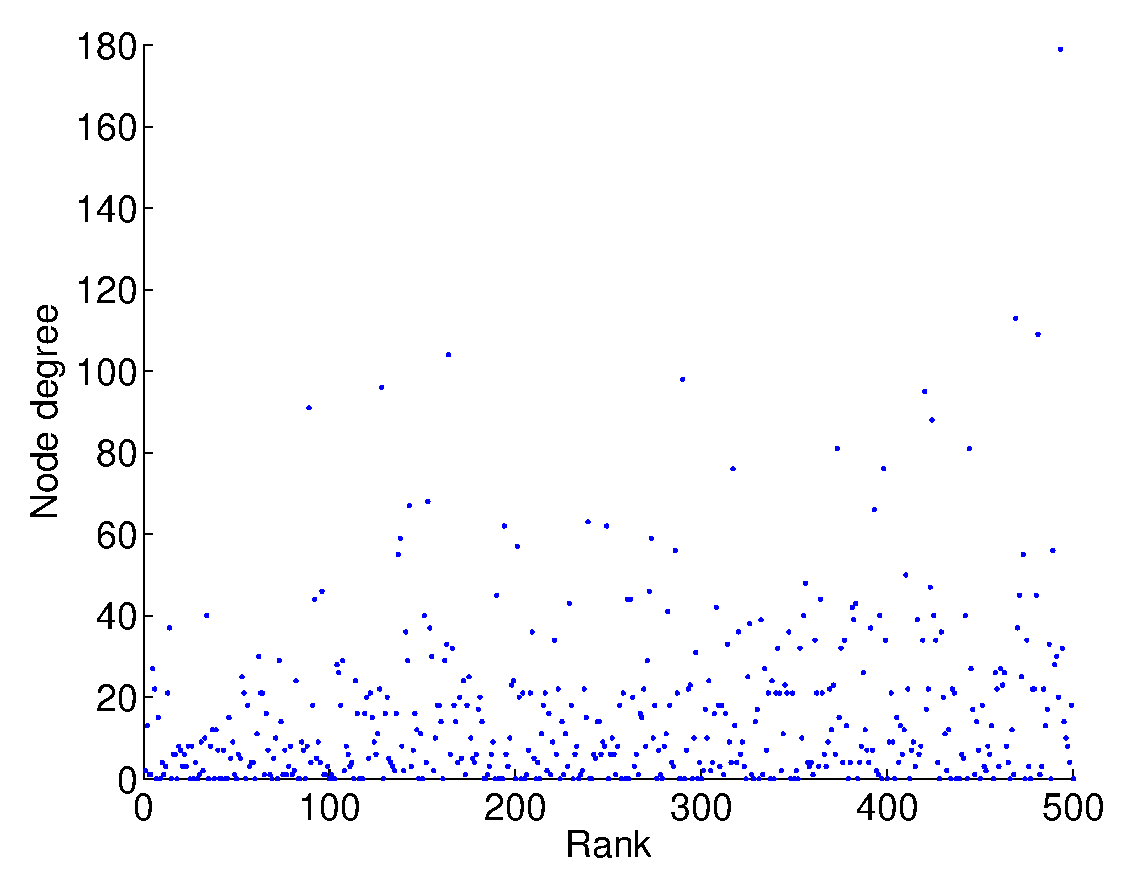
\includegraphics[width=.45\textwidth]{figures/plots/scatterplot-fpd-no-adblocker.eps}\label{fig:first_party_degree_relative_rank}} \hfill
 %\subfloat[CDF with separation of domains according to their ranks]{
 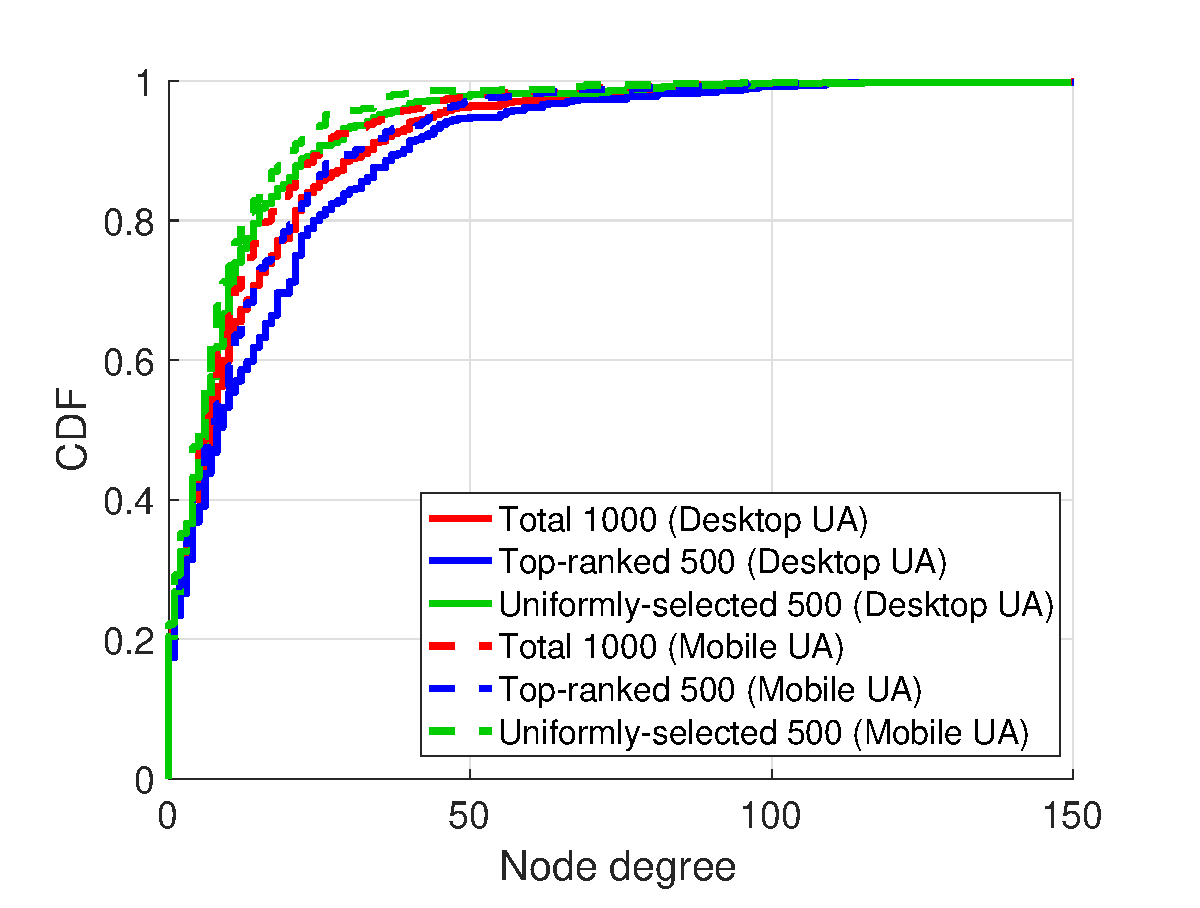
\includegraphics[width=.45\textwidth]{figures/plots/comparative-cdf-first-node-degree-no-adblocker.eps}
 %\label{fig:cdf_first_node_degree}}

 \caption{FPD node degree for the browser profiles \textit{NoAdblocker} (solid line) and \textit{NoAdblocker\_MUA} (dotted line) on 28/04/2016.}
 \label{fig:first_node_degree}
\end{figure}


%In this section we investigate the correlation between the Alexa rank of the URL and a filtering-performance metric ---i.e.\ the FPD node degree. In Figure~\ref{fig:first_party_degree_relative_rank} we plot the FPD node degree with respect to the domain rank to provide a finer visualization of the previous result, for a specific browser profile $U$ and a specific date. The figure presents only the data for the top 500-ranked websites and does not show any trend that can suggest a clear relationship between the relative rank and the node degree. Our visual observation is confirmed by the calculation of the correlation of the two parameters that yields 10.49\%.

Before investigating the effect of the different adblockers, we characterize the FPD node degree with the \textit{NoAdblocker} and \textit{NoAdblocker\_MUA} browser profiles as a baseline. Figure~\ref{fig:first_node_degree} shows the cumulative distribution function (CDF) of the FPD node degree of both profiles on a single day (28/04/2016) for the top-ranked 500 domains and the 500 uniformly-selected ones. As can be seen, in both the top 500 and the uniformly selected domains, almost 20\% of the websites did not load any third-parties at all. These domains do therefore not impose a privacy risks to the users. On the other hand, more than 80 percent of the visited domains generate requests to third parties. In general, we can say that the top 500 domains tend to generate more requests to third-parties than the uniformly selected domains, indicating that advertisement and tracking is more likely to happen on popular domains. However, even the randomly selected domains have a quite significant number of third-party requests. While the mean FPD node degree for the top 500 domains and uniformly selected domains are around 17 and 12 respectively, both FPD node degree distributions has a quite long tail. We observe a significant number of FPD node degrees above 100 with one domain in the top 500 exhibiting a degree of 180. These sites raise serious concerns in terms of privacy since each individual third-party request could potentially leak personal information of the visiting users to these third parties.

%loaded almost no third parties, while at the same time only a very limited number were accessed by more than 50 TPD nodes in all cases. Comparing the curves, we confirm that less third parties were loaded for the uniformly-selected domains, affirming the results of Figure~\ref{fig:top_last_domains_comparison}.

\subsubsection{Comparison of the Different Browser Profiles}

%\begin{figure}[!t]
% \centering
%  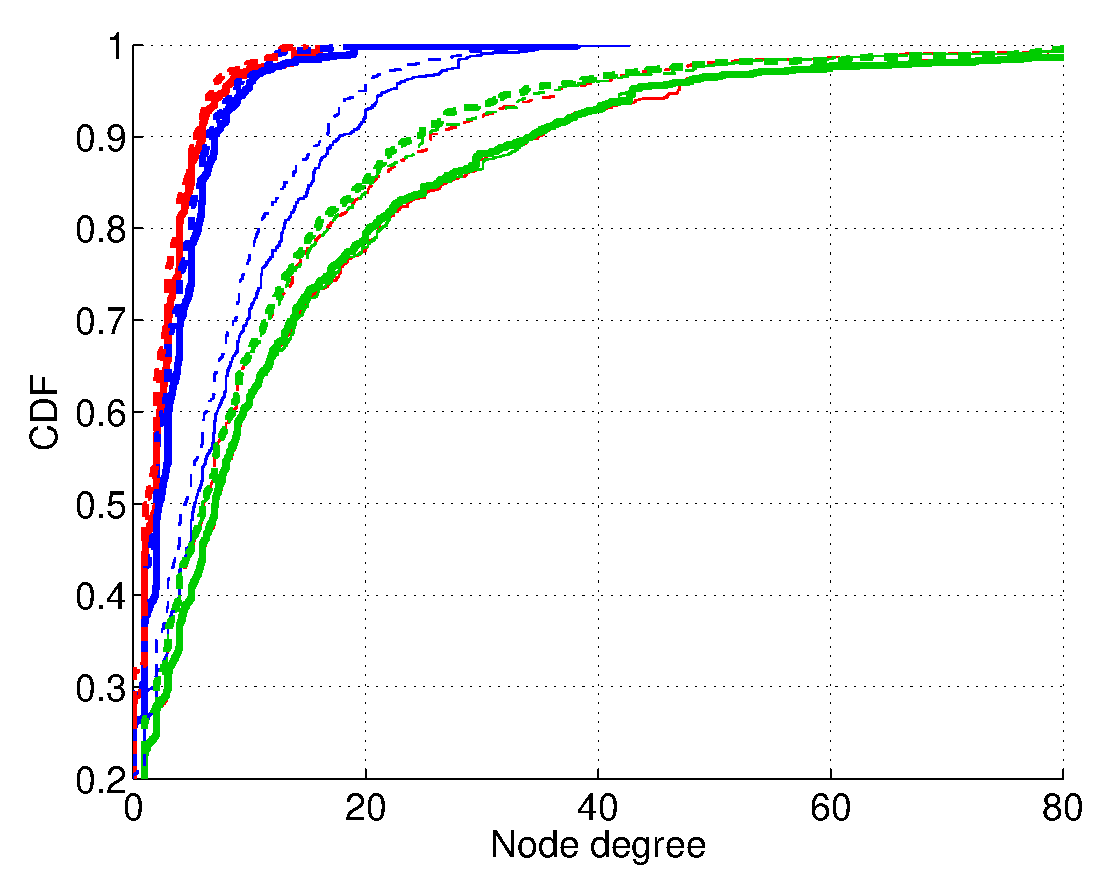
\includegraphics[width=.45\textwidth]{figures/plots/cdf-scatterplot-means.eps}
%  \caption{Mean FPD node degree across time for all browser profiles}
%  \label{fig:cdf_mean_first_node_degree}
%\end{figure}

\begin{figure*}
 \centering

 \subfloat[CDF of the average node degree over 3 weeks.]
 {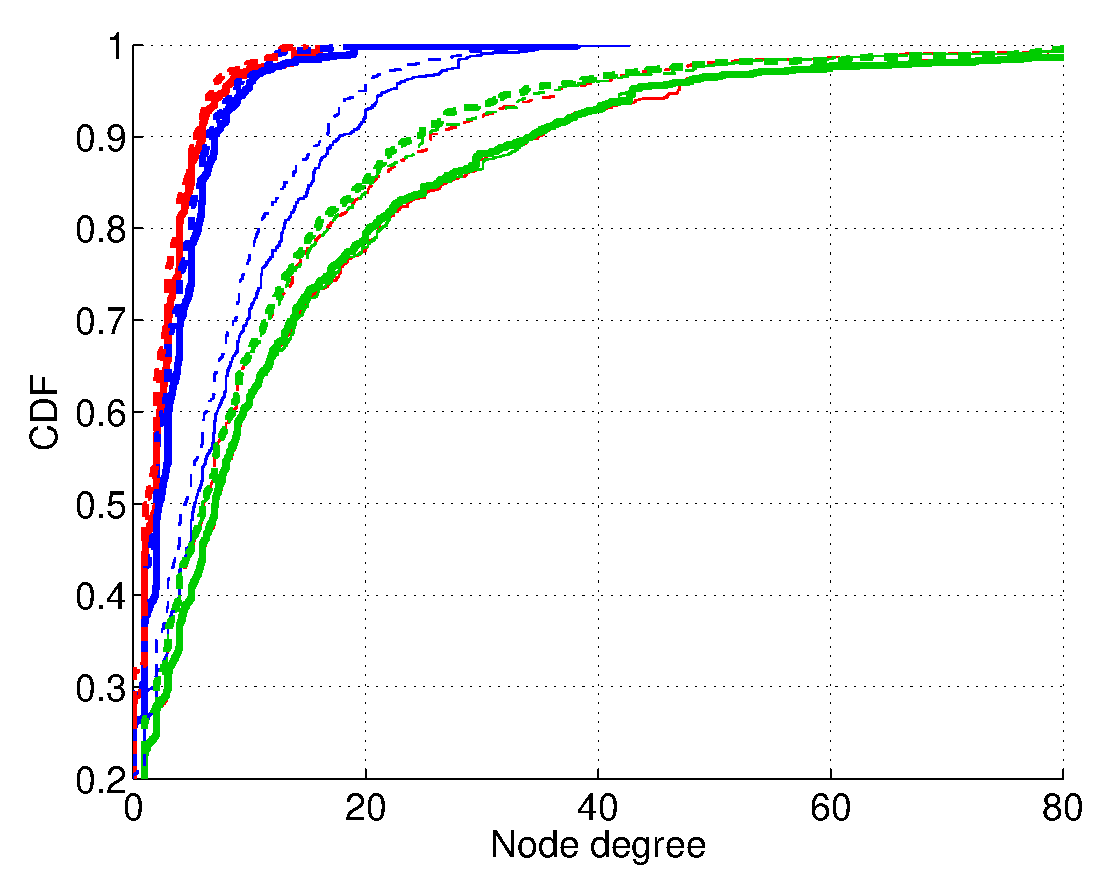
\includegraphics[width=.45\textwidth]{figures/plots/cdf-scatterplot-means.eps}\label{fig:mean_first_node_degree}} \hfill
 \subfloat[CDF of the standard deviation of the node degree over 3 weeks.]
 {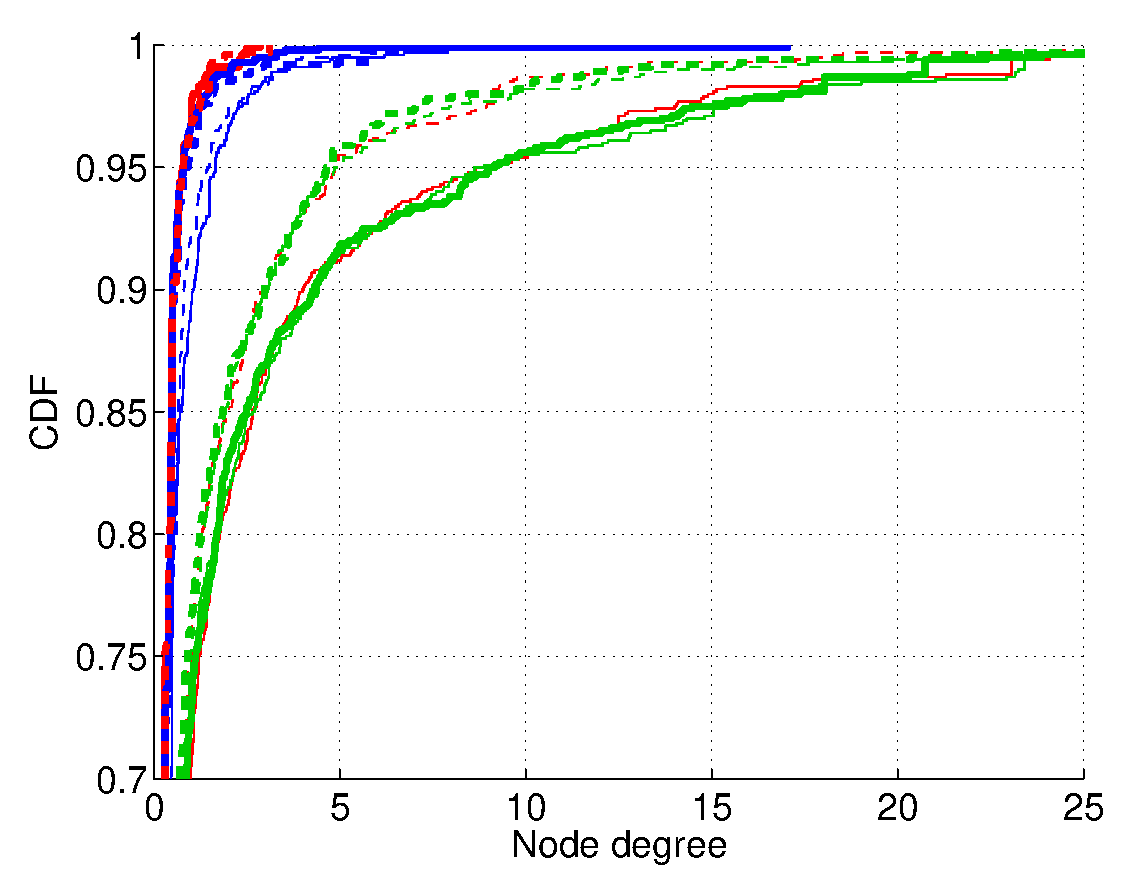
\includegraphics[width=.45\textwidth]{figures/plots/cdf-scatterplot-stdev.eps}\label{fig:std-first_node_degree}}

 \caption{FPD node degree distribution for all browser profiles. Legend is provided in Table~\ref{table:browser_profiles}.}
 \label{fig:stdev_first_node_degree}
\end{figure*}

To understand the effectiveness of the different adblockers and browser profiles at suppressing requests to third-parties, we plot in Figure~\ref{fig:stdev_first_node_degree} the FPD node degree distribution for all domains as a CDF. Figure~\ref{fig:mean_first_node_degree} shows the node degree distribution averaged over the different days while Figure~\ref{fig:std-first_node_degree} represents the standard deviation of the node degree over the same days. Our results indicate the following findings.

The worst filtering performance is achieved with the \textit{do not track} HTTP header options (\textit{NoAdblocker\_DNT} and \textit{NoAdblocker\_DNT\_MUA}) and Ghostery in default mode (\textit{Ghostery\_Default} and \textit{Ghostery\_Default\_MUA}). With these browser profile configurations, almost none of the third-party requests are blocked. AdblockPlus (\textit{Adblockplus\_Default} and \textit{Adblockplus\_Default\_MUA} with its default settings has a FPD node degree that is significantly lower than the aformentioned cases, i.e., the browser profiles with the DNT header enabled and Ghostery in its default configuration. Unsurprisingly, the browser profiles that filter the most third parties are those with adblockers configured to a maximum protection level. We observe that \textit{Ghostery\_MaxProtection} decreases the mean FPD node degree by approximately 80 \% compared to \textit{NoAdblocker}. On the other hand, the FDP node degree of Adblock Plus (\textit{AdblockPlus\_MaxProtection}) is reduced by almost 75 \% which is slightly behind the performance of Ghostery, but still significantly better than the default configuration option.

Interesting to note here is the large difference in blocking performance between the different configurations of the same adblockers. This result suggests that the privacy of the users is highly affected by a good configuration of the tools and that by default, these tools still permit a significant portion of the third-party requests.

The standard deviation of the FPD node degree over all domains is shown in~\ref{fig:std-first_node_degree}. As we can see, the profiles which have a large FPD node degree tail such as \textit{NoAdblocker}, \textit{NoAdblocker\_MUA}, \textit{NoAdblocker\_DNT}, \textit{NoAdblocker\_DNT\_MUA}, and \textit{Ghostery\_Default} also exhibit this tail in the standard deviation. However, the profiles which tend to have a small FDP node degree feature a small standard deviation as well.





%Examining the cumulative distribution function (CDF) of the FPD node degree (Figures~\ref{fig:cdf_mean_first_node_degree},~\ref{fig:stdev_first_node_degree}) we can profile the extent to which the visited URLs are being tracked by third party domains. For each FPD we calculate the mean node degree across multiple days. Afterwards, we plot the probability $$P(\textnormal{FPD node degree} \leq X)$$ of a FPD node to have a mean degree less than $X$ or, equivalently, to load on average less than $X$ TPDs. A browser profile whose corresponding curve lies on the leftmost side of the graph is expected to have a lower mean FPD node degree which is equivalent to a better filtering performance in terms of privacy.

%We conclude that the profiles \textit{Ghostery\_Default}, \textit{NoAdblocker} and \textit{NoAdblocker\_DNT} load many third parties, while Ghostery with maximum protection blocks the most TPDs.




%In Figure~\ref{fig:cdf_first_third_node_degree} we visualize the FPD and TPD node degrees for a specific date and create the CDF of the two metrics. Although the results are in accord with the conclusions of the previous plots (cf. Figures~\ref{fig:metrics_without_entities},~\ref{fig:cdf_mean_first_node_degree},~\ref{fig:cdf_stdev_first_node_degree}), it is to be observed that the FPD node degree gives us a better discerning ability with respect to the TPD node degree for profiles with similar filtering performances.

%When comparing the blocking performance of \textit{Ghostery\_\allowbreak MaxProtection} and \textit{Adblockplus\_\allowbreak MaxProtection}, we observe that  the CDF curves for the two profiles coincide for $CDF \le 0.3$ and $d \le 1$, where $d$ the node degree. This means that 30\% of the FPD nodes for one browser profile has the exact same distribution as 30\% of the FPD nodes for the other browser profile and hence we cannot tell which one of the two presents a better filtering performance by examining only this part of the curve. However, for each value of node degree, $d > 1$, the browser profile \textit{Ghostery\_\allowbreak MaxProtection} has less FPD nodes that have a node degree as high as $d$ than the browser profile \textit{Adblockplus\_\allowbreak MaxProtection} has, which can be directly translated to a better filtering performance for the profile \textit{Ghostery\_\allowbreak MaxProtection}.

%Accordingly, the better performance for the profile \textit{Ghostery\_\allowbreak MaxProtection} can be concluded similarly when we use the TPD node degree as a metric (Figure~\ref{fig:cdf-third-node-degree}). Nevertheless, the part where the two curves coincide ---and thence do not offer any comparative result--- is for $CDF \le 0.95$. As a consequence, to compare the performances of the two browser profiles, we have to examine a much smaller part of the curve, which leads to less clear conclusions.


\subsubsection{Temporal Dynamics}

%\begin{figure*}[!t]
%  \centering

%  \subfloat[Mean value of the degree of the 500 top-visited FPD nodes]{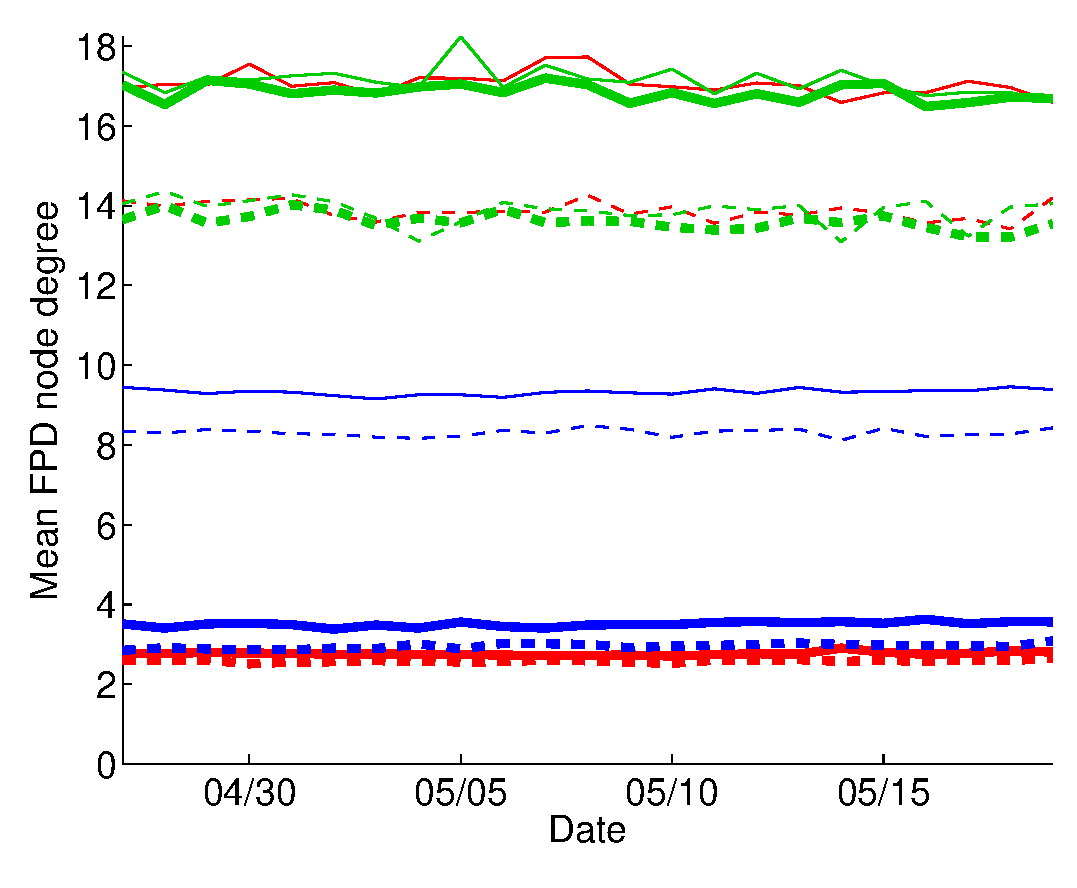
\includegraphics[width=.45\textwidth]{figures/plots/top500-first-means.eps}\label{fig:top500_first_means}} \hfill
  %\subfloat[Mean value of the degree of the 500 uniformly-selected FPD nodes]{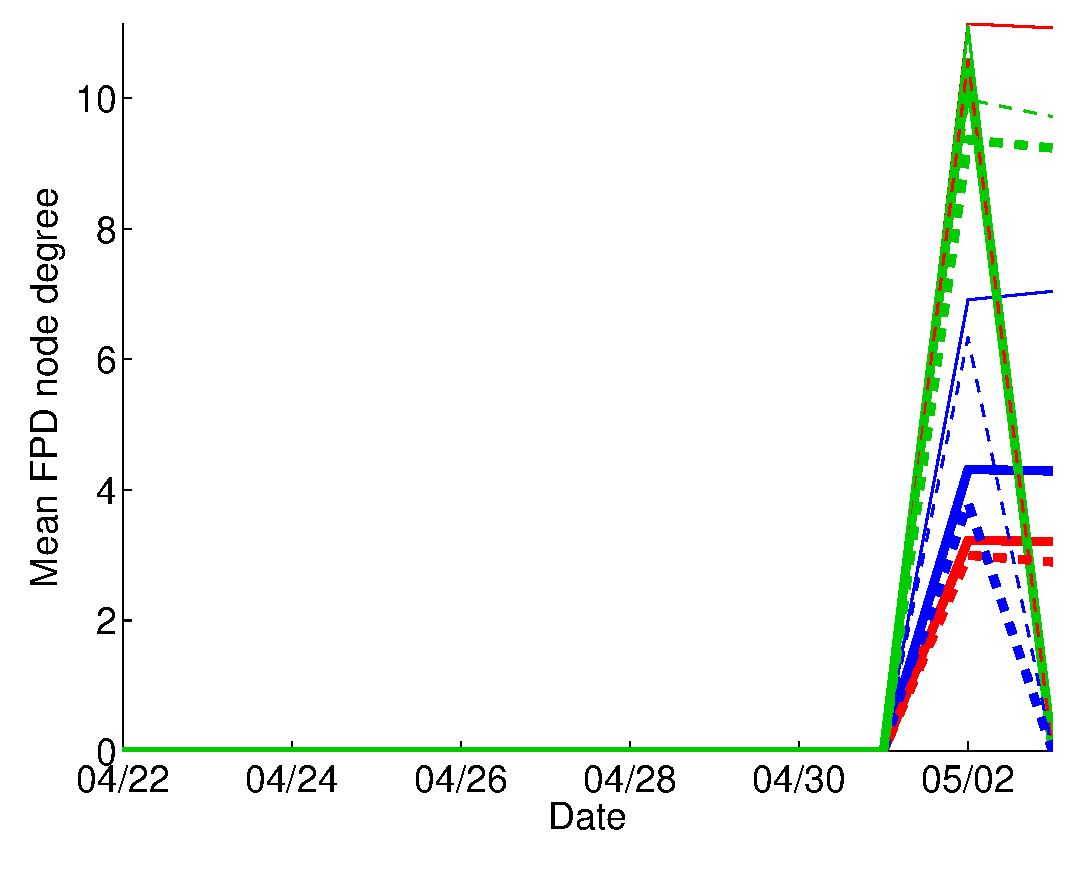
\includegraphics[width=.45\textwidth]{figures/plots/last500-first-means.eps}\label{fig:top500_random_means}}

%  \caption{Comparison of the filtering performance of the browser profiles $U$ when tested the top-visited domains and the uniformly-selected ones.}
%  \label{fig:top_last_domains_comparison}
%\end{figure*}

\begin{figure*}
   \centering
   \subfloat[Mean FPD over the top 500 domains.]{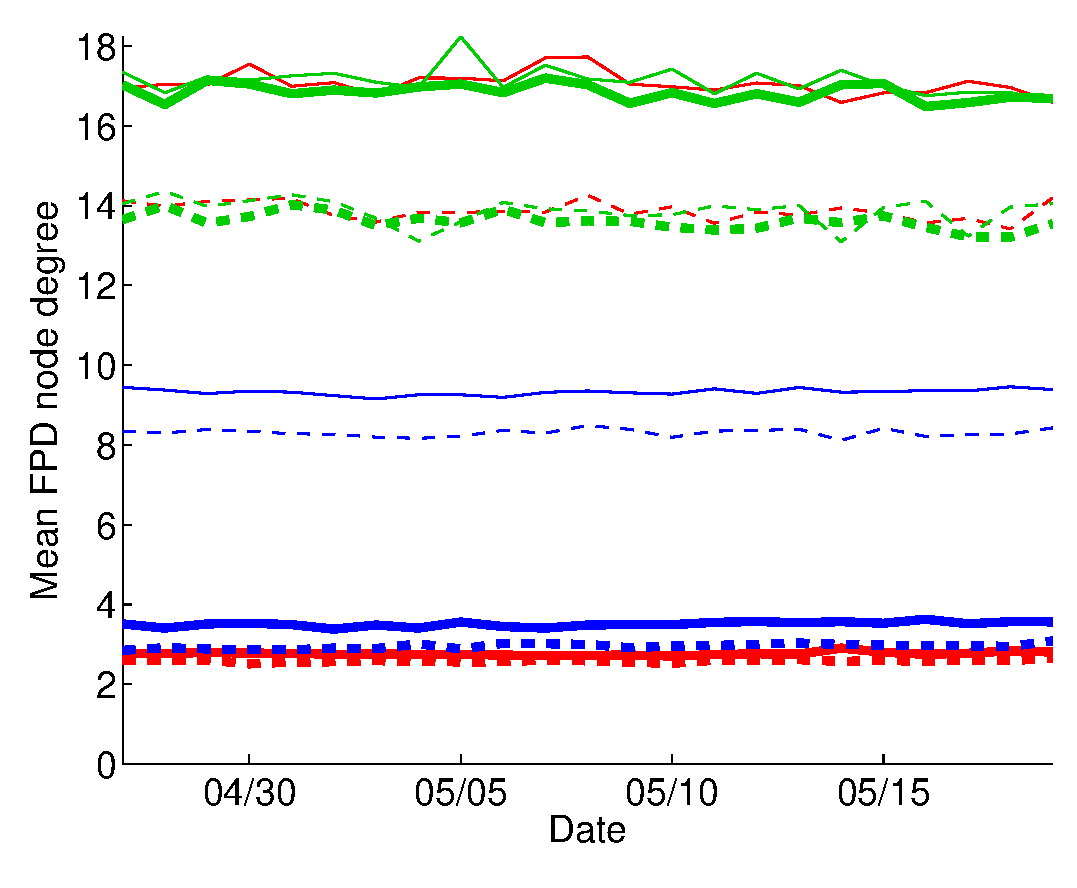
\includegraphics[width=.45\textwidth]{figures/plots/top500-first-means.eps}\label{fig:top500_first_means}} \hfill
  \subfloat[Mean FPD over the 500 uniformly-selected domains.]{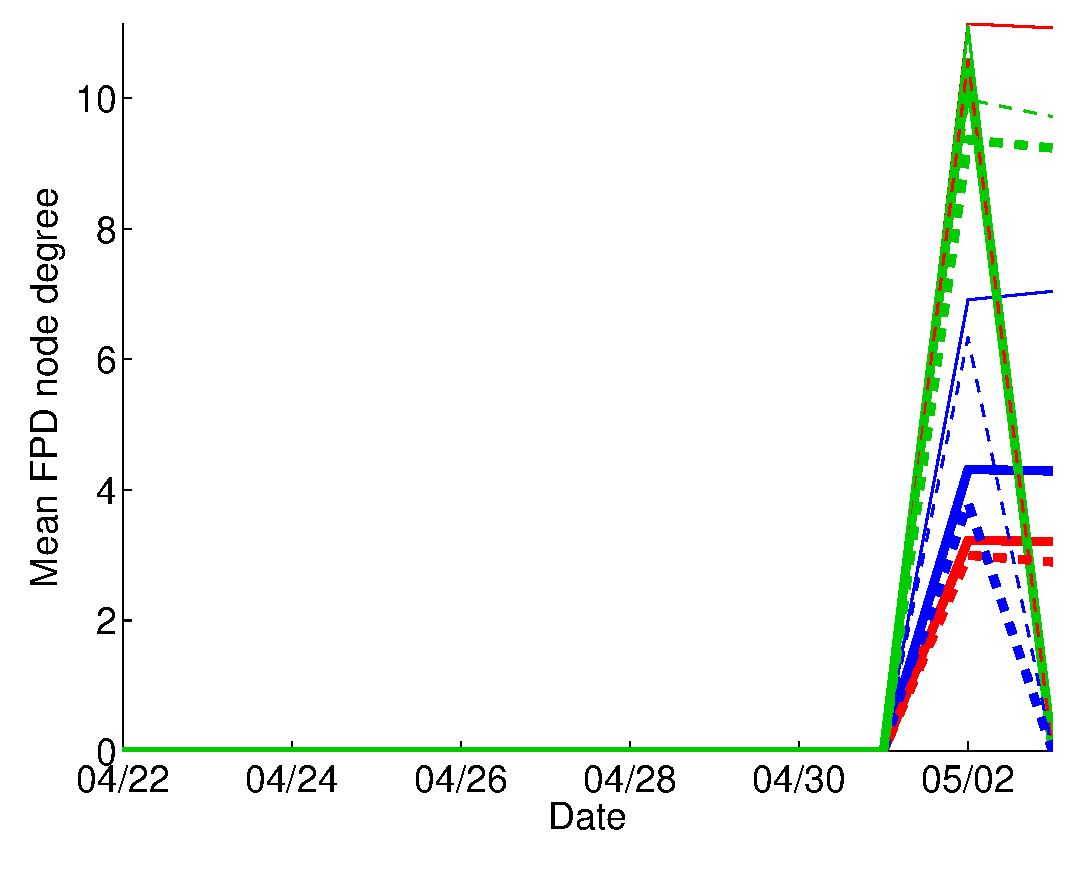
\includegraphics[width=.45\textwidth]{figures/plots/last500-first-means.eps}\label{fig:top500_random_means}} \\
   \subfloat[Maximum FPD over all visited domains.]{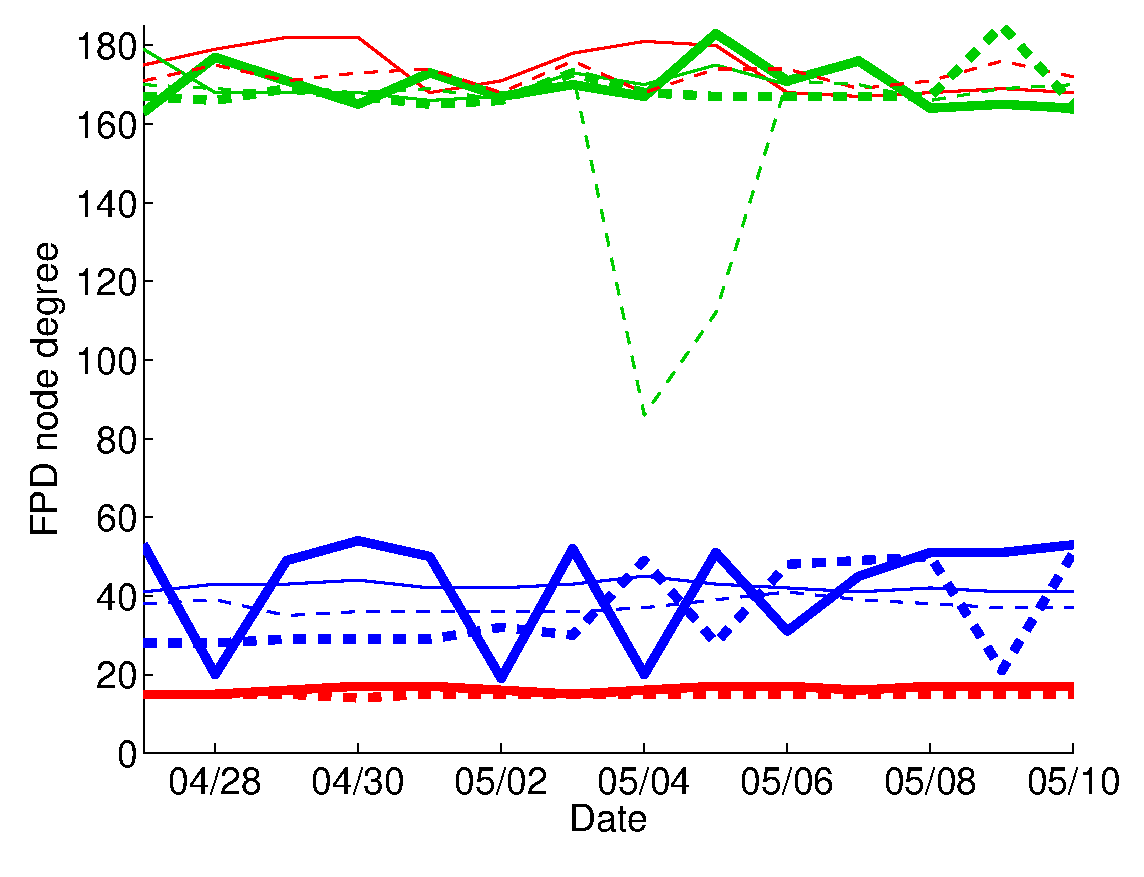
\includegraphics[width=.45\textwidth]{figures/plots/first-mean-top1.eps}\label{fig:first_mean_top1_without_entities}} \hfill
   \subfloat[Mean FPD over the 10 domains with the highest FPD from all visited domains.]{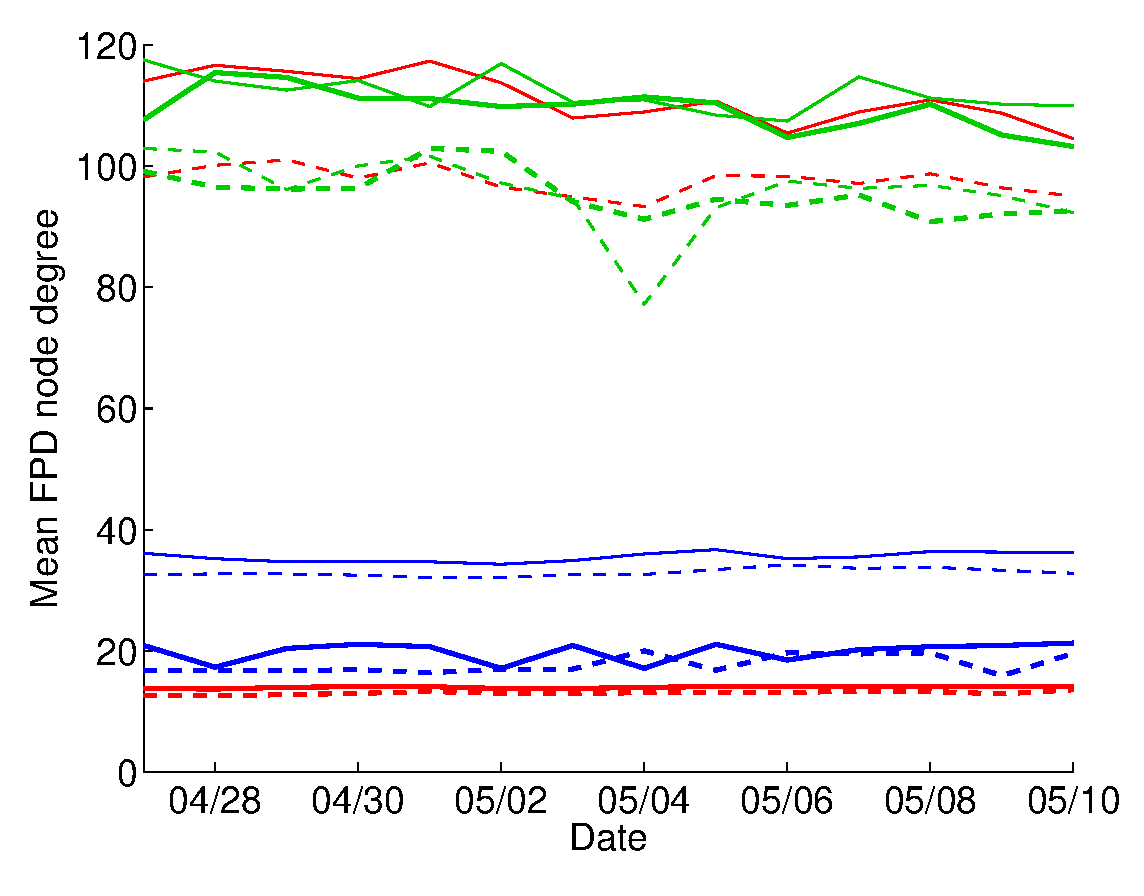
\includegraphics[width=.45\textwidth]{figures/plots/first-mean-top10.eps}\label{fig:first_mean_top10_without_entities}}

  \caption{Evolution over time of the first party node degree (FPD). Legend is provided in Table~\ref{table:browser_profiles}.}
  \label{fig:FPD_over_time}

\end{figure*}


To capture the temporal dynamics of third-party requests, we plot in Figure~\ref{fig:FPD_over_time} the FPD over time in the considered period of 3 weeks. Figure~\ref{fig:top500_first_means} and \ref{fig:top500_random_means} show the mean FPD for the top 500 domains and the uniformly selected domains respectively. We observe a quite stable temporal evolution over the individual days for both datasets. In particular, in none of the datasets, we can observe a change in relative order between the different browser profiles. We can therefore conclude that in general, the privacy of the users is not sensitive to web site or blacklist optimizations that happen at shorter time scales.

To check whether this conclusion also translates to individual domains, we take a closer look at the domains with the highest FPD in Figure~\ref{fig:first_mean_top1_without_entities} and \ref{fig:first_mean_top10_without_entities}. Figure~\ref{fig:first_mean_top1_without_entities} shows the evolution of the FPD for the domain with the highest FPD in any of the dataset while Figure~\ref{fig:first_mean_top10_without_entities} represents the mean of the FPD over the ten domains with the highest FPD. We make two interesting observations here. First, the domains with the largest FPDs tend to exhibit a higher variation over different days. In particular, for \textit{Ghostery\_Default} and \textit{Ghostery\_Default\_MUA} in Figure~\ref{fig:first_mean_top1_without_entities}, the filtering of third-party requests shows a larger fluctuation over time. Also, \textit{AdblockPlus\_MaxProtection} and \textit{AdblockPlus\_MaxProtection\_MUA} has a significantly higher fluctuation for the top domain than on average. Second, the filtering performance of the different browser profiles is more clustered than it is was on average for all the domains. For example, on most days, the performance of \textit{Ghostery\_Default} and \textit{Ghostery\_Default\_MUA} is almost identical to \textit{NoAdblocker}, while those two profiles where significantly outperforming the \textit{NoAdblocker} profile in Figures~\ref{fig:top500_first_means} and \ref{fig:top500_random_means}. These two observations indicate that these domains with a high FPD score could be more active at circumventing blocking strategies by adblockers.

\subsection{How do Adblockers Reduce the Tracking Range of Third-party Domains?}

\begin{figure}
  \centering
  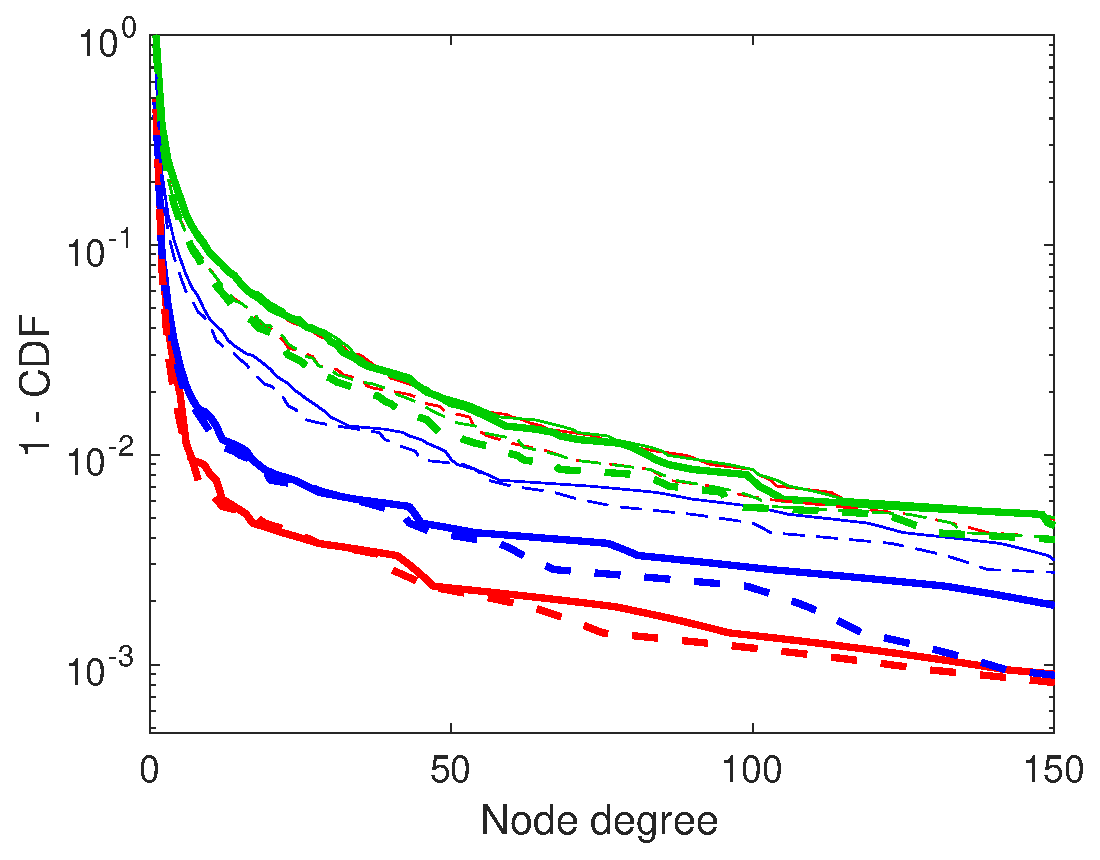
\includegraphics[width=.45\textwidth]{figures/plots/cdf-third-node-degree.eps}
  %\subfloat[Top 500 domains (!!Bild als Platzhalter!!)).]{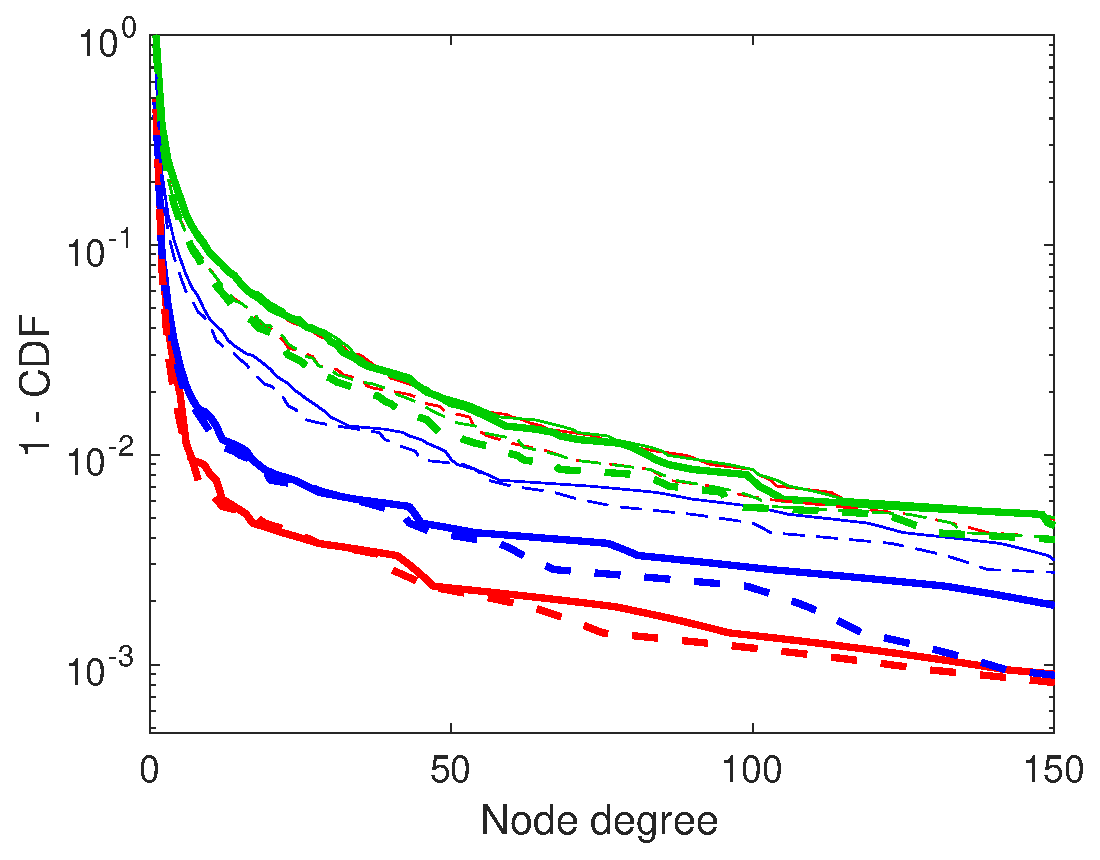
\includegraphics[width=.45\textwidth]{figures/plots/cdf-third-node-degree.eps}\label{fig:cdf-third-node-degree}}
  %\subfloat[Uniformly selected domains. (!!Bild als Platzhalter!!)]{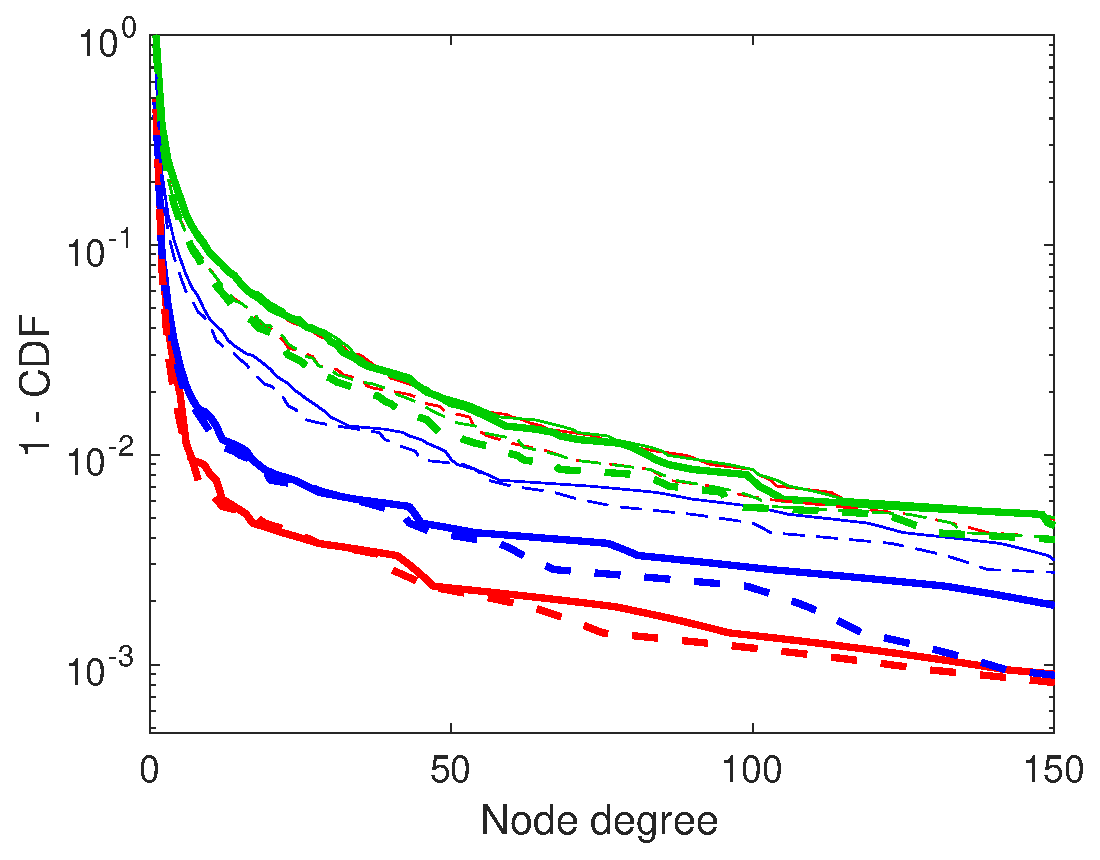
\includegraphics[width=.45\textwidth]{figures/plots/cdf-third-node-degree.eps}\label{fig:cdf-third-node-degree}}
  \caption{Inverse CDF of TPD node degree for all browser profiles.}
  \label{fig:cdf_first_third_node_degree}
\end{figure}

  \begin{table}
  \centering
  \begin{tabular}{|c|c|c|c|c|c|}
  \hline
    \multirow{2}{*}{Third-Party Domain} & \multirow{2}{*}{Legal Entity} & \multicolumn{3}{|c|}{TPD Degree} \\
  \cline{3-5}
    & & \scriptsize{None} & \scriptsize{Ghostery} & \scriptsize{AdblockPlus} \\
  \hline
  doubleclick.net & Google Inc. & 486 & 0 & 1 \\
  google-analytics.com & Google Inc. & 476 & 4 & 0 \\
  google.com & Google Inc. & 383 & 93 & 144 \\
  facebook.com & Facebook Inc. & 318 & 5 & 164 \\
  gstatic.com & Google Inc. & 308 & 226 & 235 \\
  googlesyndication.com & Google Inc. & 204 & 0 & 0 \\
  google.ch & Google Inc. & 189 & 0 & 0 \\
  fonts.googleapis.com & Google Inc. & 185 & 145 & 141 \\
  adnxs.com & AppNexus Inc. & 159 & 0 & 0 \\
  facebook.net & Facebook Inc. & 157 & 0 & 140 \\
  \hline
  \end{tabular}
  \caption{Top-loaded TPDs for browser profile \textit{NoAdblocker} and the corresponding values for Ghostery and AdblockPlus with maximum-protection settings (browser profiles \textit{Ghostery\_MaxProtection} and \textit{AdblockPlus\_MaxProtection}) on 28/04/2016}
  \label{table:top_10_third_party_domains}
  \end{table}


In order to understand the extend to which individual third-parties are able to track users while surfing across different domains, we look next at the degree of third-party domains (TPD). The TPD degree reflects how many visits to different first-party domains an individual third-party can observe.  Figure~\ref{fig:cdf_first_third_node_degree} shows how the different browser profiles affect the TPD degree of all third-parties that we encountered in our experiments. As we can see, the TPD is highly skewed. %90 percent of the third-parties have a TPD of less than 10 for the \textit{NoAdblocker} profile while the largest TPD degree we observe is 486
Only 10~percent of the third-parties have a TPD of more than 10 for the \textit{NoAdblocker} profile while the largest TPD degree we observe is 486 (\textit{None} column of Table~\ref{table:top_10_third_party_domains}).
In general, we can therefore say that a small number of third-party domains are able to capture the vast majority of the visits to first parties.

Considering the effect of the different browser profiles, we observe a similar trend as for the FPD degree. The \textit{Ghostery\_MaxProtection} and \textit{AdblockPlus\_MaxProtection} profiles manage to effectively reduce the TPD node degree of all domains. However, in their default settings, AdblockPlus and Ghostery have only a noticeable effect on the domains with a small TPD degree, while these profiles have almost no impact on the filtering performance of domains with a large TPD node degree. Again, the browser profiles with the Do Not Track option enabled result in similar TPD node degrees as without the option.

In Table~\ref{table:top_10_third_party_domains}, we list the 10 domains with the highest TPD node degree (when no adblocker is applied) and compare how these numbers decrease with the \textit{Ghostery\_MaxProtection} and \textit{AdblockPlus\_MaxProtection} browser profiles. Ghostery achieves generally better performance, although AdblockPlus outperforms marginally Ghostery for 2 domains. Interesting to notice here is that some third-party domains from this list still exhibit a high TPD node degree with any of the adblockers enabled. These are the domains google.com, gstatic.com, and fonts.googleapis.com. These domains provide important content to render the web pages of the first parties and can therefore not be blocked. The other domains relate to advertisements, tracking, and social media and their TPD degrees are effectively reduced by Ghostery. AdblockPlus is not so effective at reducing the TPD degree of domains such as facebook.com and facebook.net.

%We observe that, 7 out of 10 of these TPDs belong to the same legal entity, i.e. \textit{Google Inc.}. The two other entities that appear in the list are \textit{Facebook Inc.} and \textit{AppNexus Inc.}, thus confirming the results the Table~\ref{table:top_10_tpd_entities}, where the three first places are occupied by the exact same legal entities.


\subsection{How do Adblockers Reduce the Tracking Range of Legal Entities?}


\begin{table}
  \centering
  \begin{tabular}{|c|c|c|c|c|}
  \hline
  \multirow{2}{*}{Legal Entity} & \multicolumn{3}{|c|}{Degree} \\
  \cline{2-4}
    & \scriptsize{None} & \scriptsize{Ghostery} & \scriptsize{AdblockPlus} \\
  \hline
  Google Inc. & 666 & 328 & 354 \\
  Facebook Inc. & 328 & 6 & 211 \\
  AppNexus Inc. & 159 & 0 & 0 \\
  TMRG Inc. & 143 & 0 & 4 \\
  Twitter Inc. & 137 & 9 & 87 \\
  Oracle Corporation & 123 & 2 & 39 \\
  Adobe Systems Incorporated & 107 & 6 & 32 \\
  Yahoo! Inc. & 99 & 7 & 5 \\
  AOL Inc. & 88 & 3 & 3 \\
  OpenX Technologies & 88 & 0 & 0 \\
  \hline
  \end{tabular}
  \caption{Legal entities with the highest TPE node degree for browser profile \textit{NoAdblocker} and the corresponding values for Ghostery and AdblockPlus with maximum-protection settings (browser profiles \textit{Ghostery\_MaxProtection} and \textit{AdblockPlus\_MaxProtection}) on 28/04/2016.}
  \label{table:top_10_tpd_entities}
  \end{table}


As we have seen in Table~\ref{table:top_10_third_party_domains}, the TPD degree of many domains was effectively reduced with adblockers, but some domains still remain with a high TPD node degree, mostly in order to provide useful content when rendering the page of the FPD. As a next step, we aim to understand how adblockers reduce the tracking range at the level of legal entities. A legal entity may acquire multiple domains and therefore still receive a lot of third-party requests despite some of its domains being blocked by the adblockers.



Table~\ref{table:top_10_tpd_entities} summarizes the 10 legal entities with the highest TPD node degree, i.e.\ that were present on most of the visited URLs when the default Browser settings were applied (\textit{NoAdblocker}). As the data suggests, domains owned by \textit{Google Inc.} are loaded by 674 out of the 1000 URLs visited, thus having the most frequent presence among the rest of the third-party entities. Followed by Google Inc. are Facebook Inc., AppNexus Inc., and TMRG Inc. with node degrees of 328, 159, and 143 respectively. The degree of the following domains then quickly drops below 100.

Also presented in Table~\ref{table:top_10_tpd_entities} is the node degree of the top 10 legal entites with the \textit{Ghostery\_MaxProtection} and \textit{AdblockPlus\_MaxProtection} browser profiles enabled. Except for Google Inc., Ghostery is able to suppress the node degree of all top 10 legal entities below 10. Google Inc. however remains with a node degree of 328, meaning that despite using Ghostery, Google Inc. is able to track more than 30 percent of the page visits to the FPDs. AdblockPlus is significantly less effective than Ghostery even in the maximum protection mode. Still, it reduces significantly the TPD node degree for most TPDs.


%The relative presence among the entities can be directly compared by their normalized degree, that is, the FPD node degree of the entity divided by the maximum FPD node degree found in our experiments ---in this case the degree of the entity \textit{Google Inc.}.


\subsection{Geographical Considerations}


  \begin{table}
  \centering
  \begin{tabular}{|c|c|}
  \hline
  Country & First-Party Entities \\
  \hline
  United States & 35.7 \% \\
  Canada & 7.4 \% \\
  Japan & 4.8 \% \\
  Switzerland & 4.0 \% \\
  Germany & 3.8 \% \\
  India & 3.5 \% \\
  Great Britain & 3.0 \% \\
  Russia & 2.6 \% \\
  France & 2.6 \% \\
  Panama & 2.0 \% \\
  \hline
  \end{tabular}
  \caption{Countries hosting the highest percentage First-Party Entities}
  \label{table:top_10_first_party_countries}
  \end{table}

  \begin{table}
  \centering
  \begin{tabular}{|c|c|c|c|}
  \hline
  \multirow{2}{*}{Country} & \multicolumn{3}{|c|}{Third-Party Entities} \\
  \cline{2-4}
  & \scriptsize{None} & \scriptsize{Ghostery} & \scriptsize{AdblockPlus} \\
  \hline
  United States & 784 (45\%) & 483 (42\%) & 500 (45\%) \\
  Germany & 106 (6\%) & 40 (4\%) & 34 (3\%) \\
  China & 82 (5\%) & 70 (6\%) & 67 (6\%) \\
  Japan & 80 (5\%) & 62 (5\%) & 61 (6\%) \\
  Great Britain & 77 (4\%) & 43 (4\%) & 44 (4\%) \\
  France & 69 (4\%) & 33 (3\%) & 31 (3\%) \\
  Canada & 49 (3\%) & 33 (3\%) & 28 (3\%) \\
  India & 46 (3\%) & 38 (3\%) & 38 (3\%) \\
  Panama & 41 (2\%) & 32 (3\%) & 25 (2\%) \\
  Turkey & 32 (2\%) & 27 (2\%) & 27 (2\%) \\
  \hline
  Total & 2908 & 1866 & 1812 \\
  Found & 1748 (60.1\%) & 1140 (61.1\%) & 1097 (60.5\%) \\
  \hline
  \end{tabular}
  \caption{Countries hosting the highest percentage TPEs when no adblocker is used (browser profile \textit{NoAdblocker}), and the corresponding percentages when Ghostery and AdblockPlus are used under maximum protection settings (browser profiles \textit{Ghostery\_MaxProtection} and \textit{Adblockplus\_MaxProtection}) on 28/04/2016.}
  \label{table:top_10_third_party_countries}
  \end{table}



\begin{figure*}[!t]
 \centering
  \subfloat[Third-party legal entity locations]{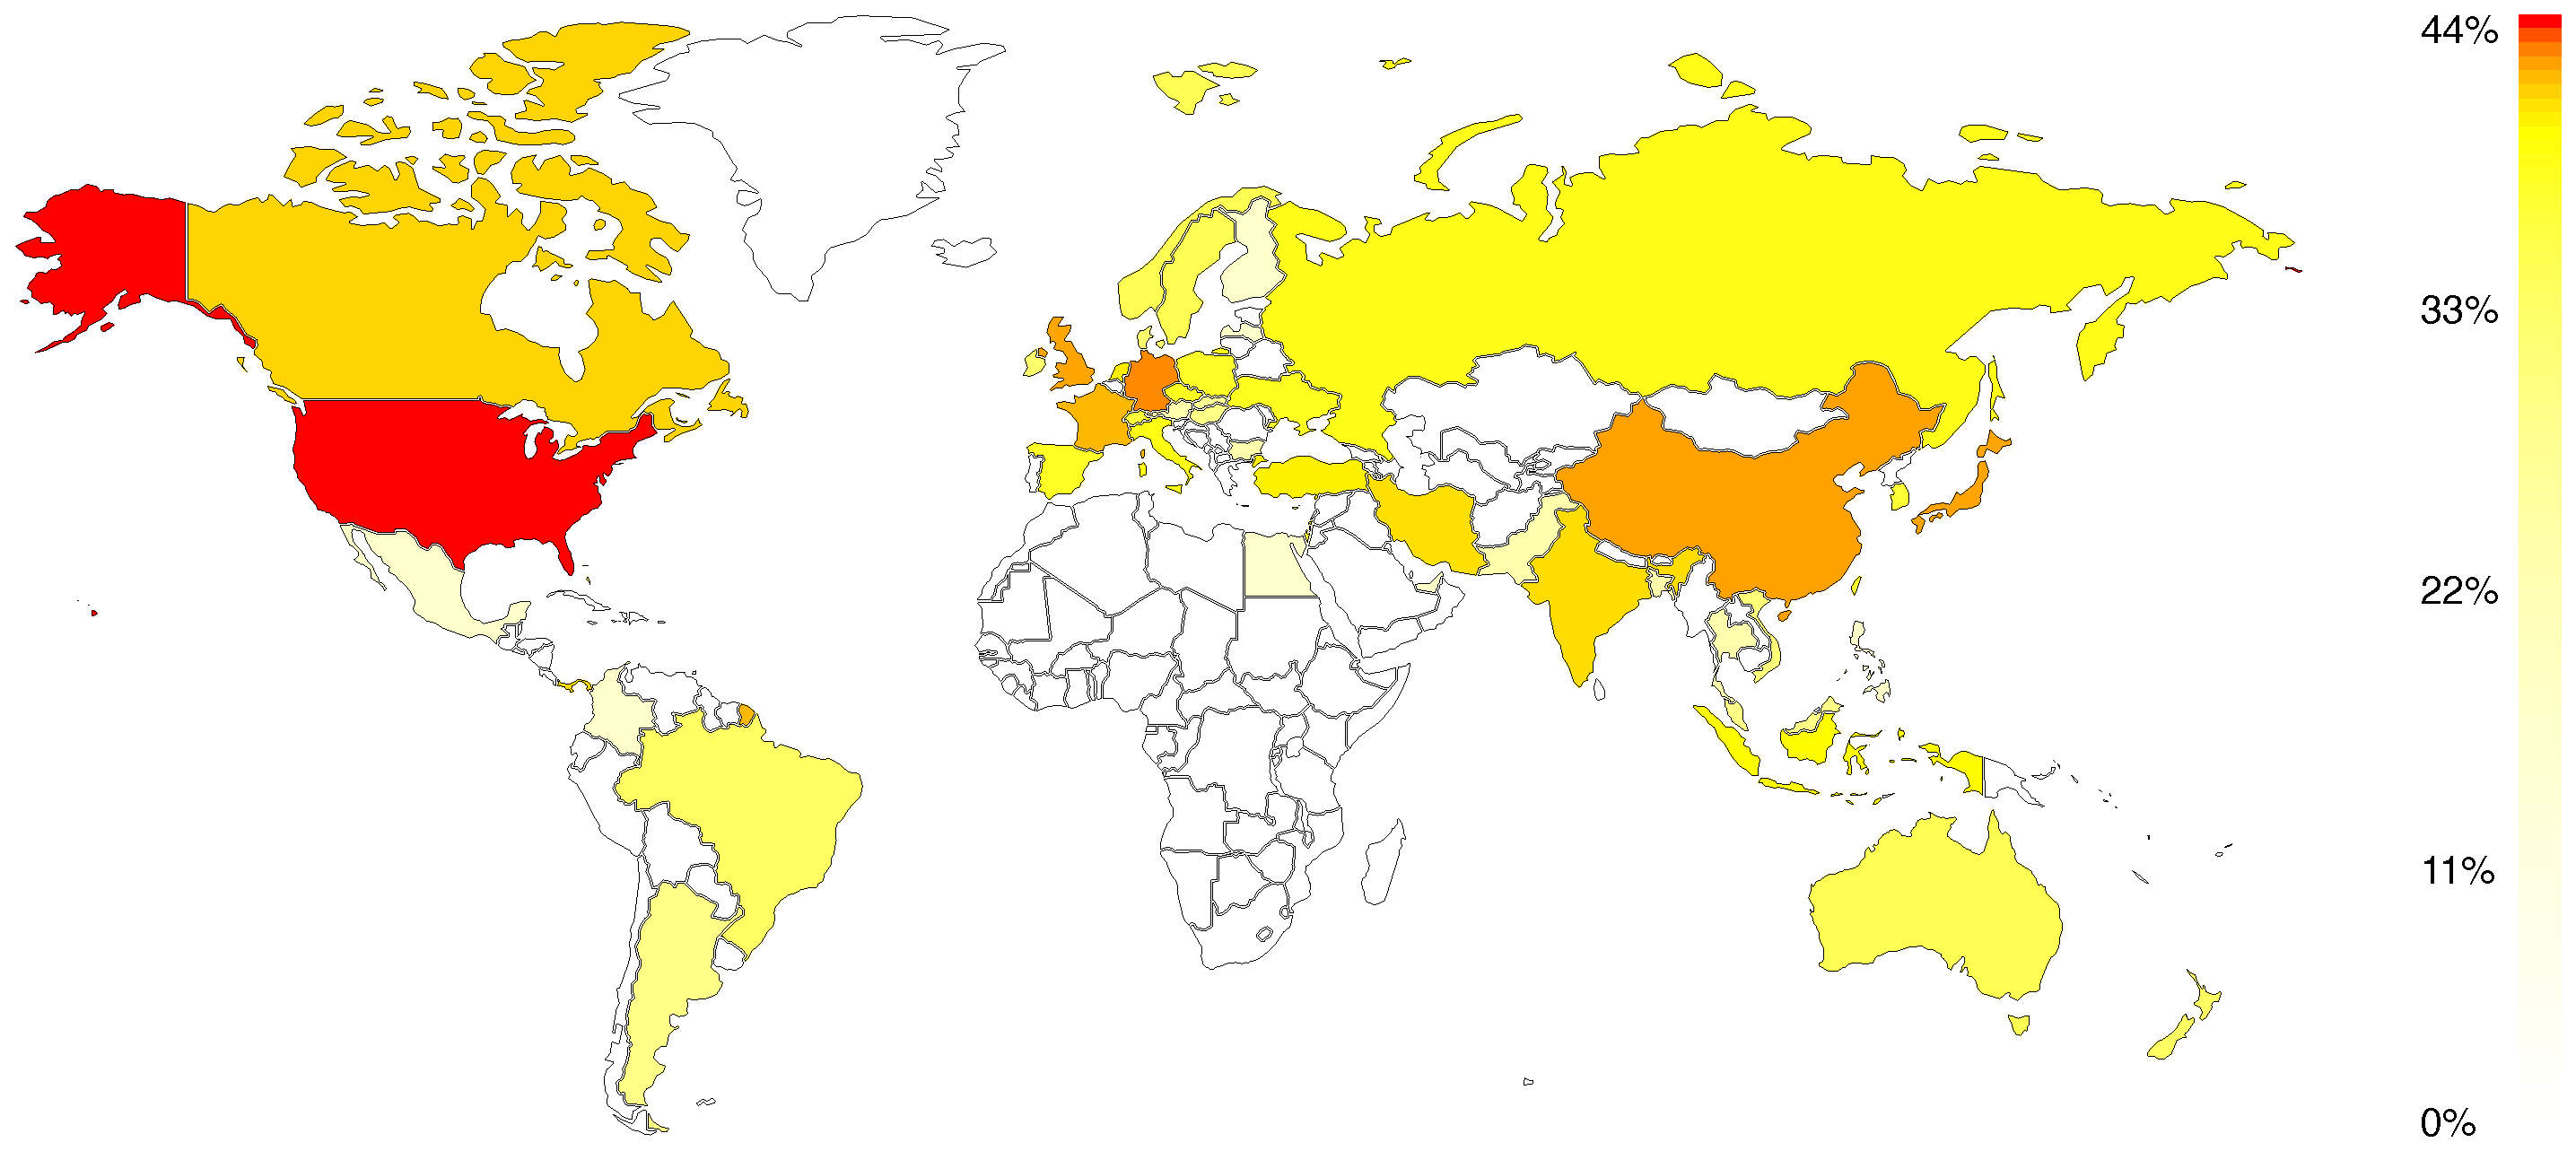
\includegraphics[width=.45\textwidth]{figures/third_party_entity_map.eps}\label{fig:third_party_entity_map}} \hfill
  \subfloat[Third party server locations]{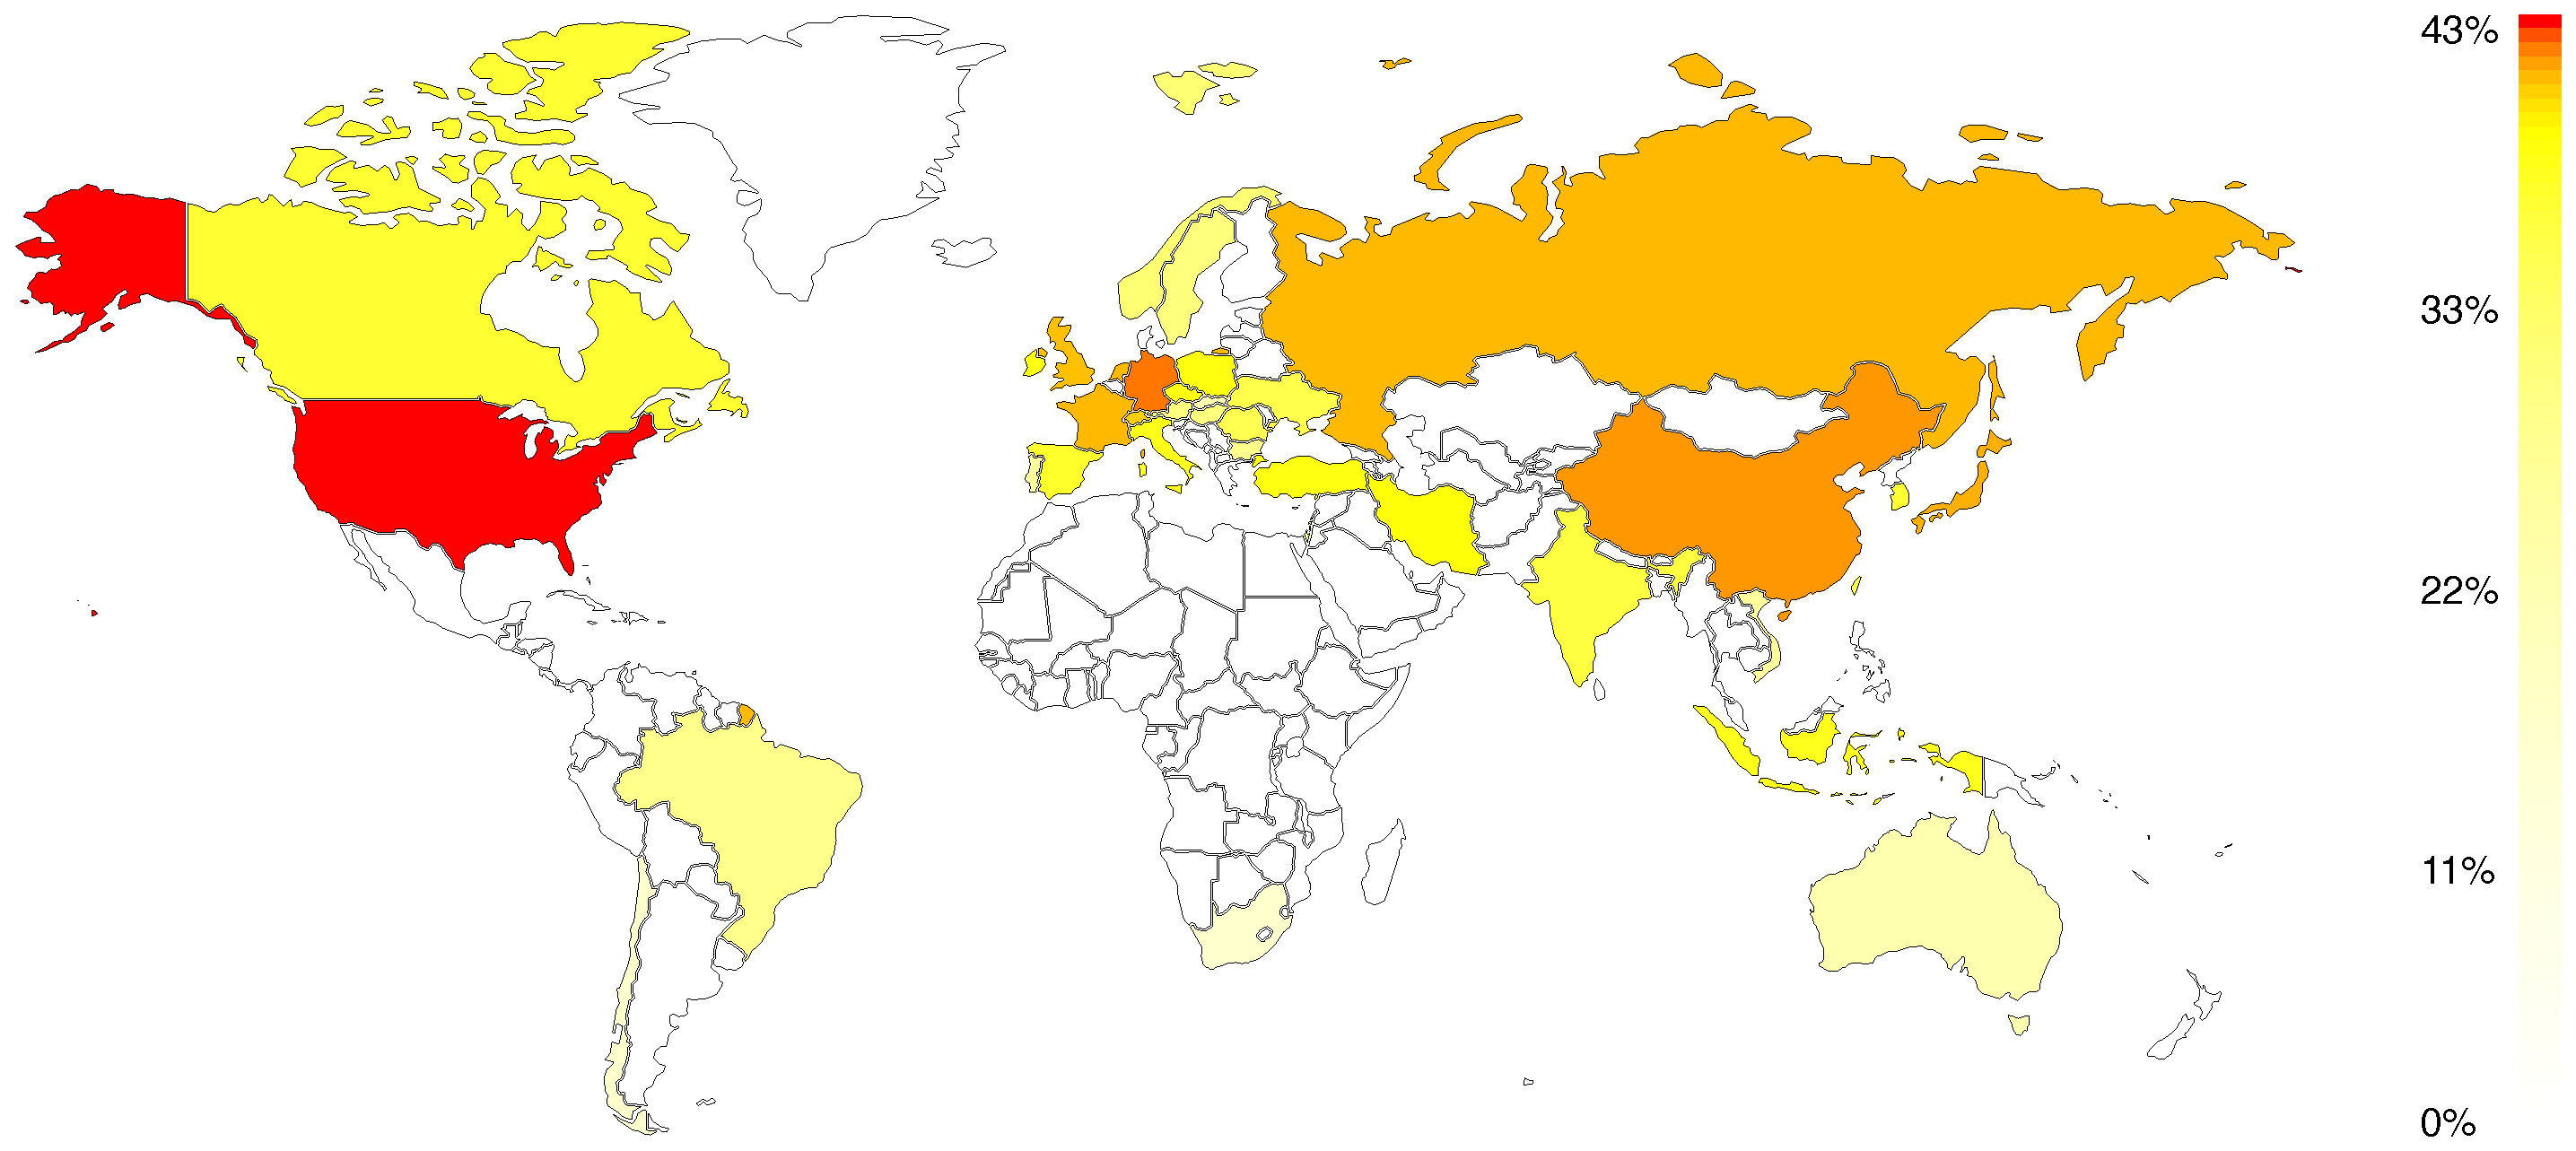
\includegraphics[width=.45\textwidth]{figures/third_party_server_map.eps}\label{fig:third_party_server_map}}
 \caption{World map depicting the locations of the legal entities and the servers for the third parties loaded during our experiments.}
\end{figure*}


Another key privacy dimension is the geographical location to which third-party requests are transferred to since local regulations govern what legal entities may do with the personal data that they collect about users. Table~\ref{table:top_10_first_party_countries} lists the 10 countries with the highest number of legal entities acting as first party in our traces. The country with the most first parties is the United States (35.7\%) followed by Canada (7.4\%) and Japan (4.8\%).  Figure~\ref{fig:third_party_entity_map} visualizes the relative number of legal entities acting as third parties in each country.  The darkest regions (red) are the countries with the most TPEs loaded, while the white ones host none of the TPEs found in our graphs. As we would expect, the USA hosts most of the first and third-party domains, while regions such as Africa or Latin America contain very few TPEs.

A more detailed view of the number of TPEs hosted by the top 10 countries is presented in Table~\ref{table:top_10_third_party_countries}. For each row, the absolute numbers refer to the TPDs that were recognized and assigned to a TPE for the specific country, while the percentages refer to the ratio of these TPEs over the total number of TPEs that were recognized by our automated script. In this table, we compare the TPEs hosted by each of these countries (column \textit{None}) to the number of TPEs loaded when the adblockers Ghostery and AdblockPlus are deployed under maximum-protection settings (columns \textit{Ghostery} and \textit{AdblockPlus}).

Interesting to note here is the difference in rank between countries in terms of legal entities that act as first and third parties. For example, China does not appear in the top ten list of countries for first parties, but ranks third in the ranking for legal entities that act as third-parties. This indicates that China hosts in relation to the other countries more third-party domains than first-party domains. The opposite is true for Switzerland and Russia which rank 4th and 7th in the ranking for first-party entities but don't appear in the top ten of third-party entities. Regarding the effect of the Ghostery and AdblockPlus, we can see that these adblockers do not significantly affect the overall distribution and ranking of the third-party legal entities. All countries experience a diminishing number of third-party legal entities that is in proportion relatively equal.



\subsection{Graph Density}

  \begin{figure}
   \centering
% \subfloat[Mean value of the degree of the FPD nodes over time for each browser profile $U$]{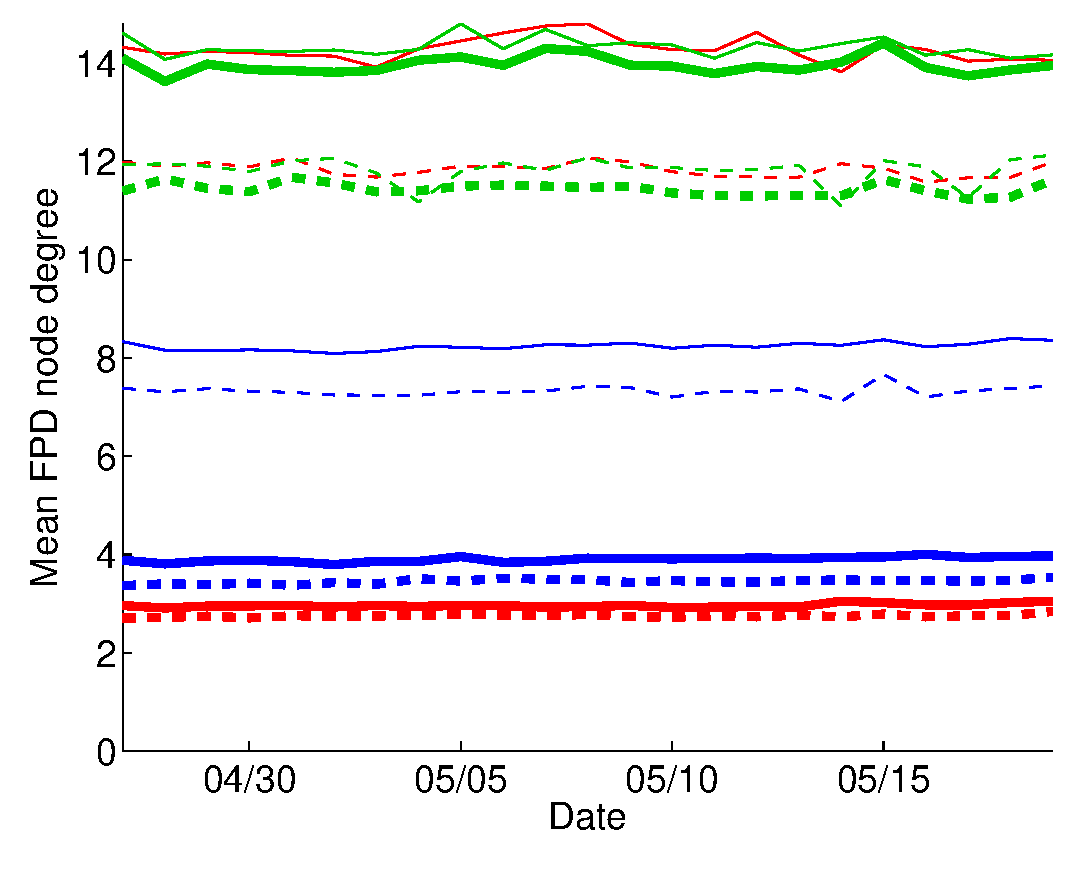
\includegraphics[width=.45\textwidth]{figures/plots/first-means.eps}\label{fig:first_means}}
 % \subfloat[Mean TPD node degree]{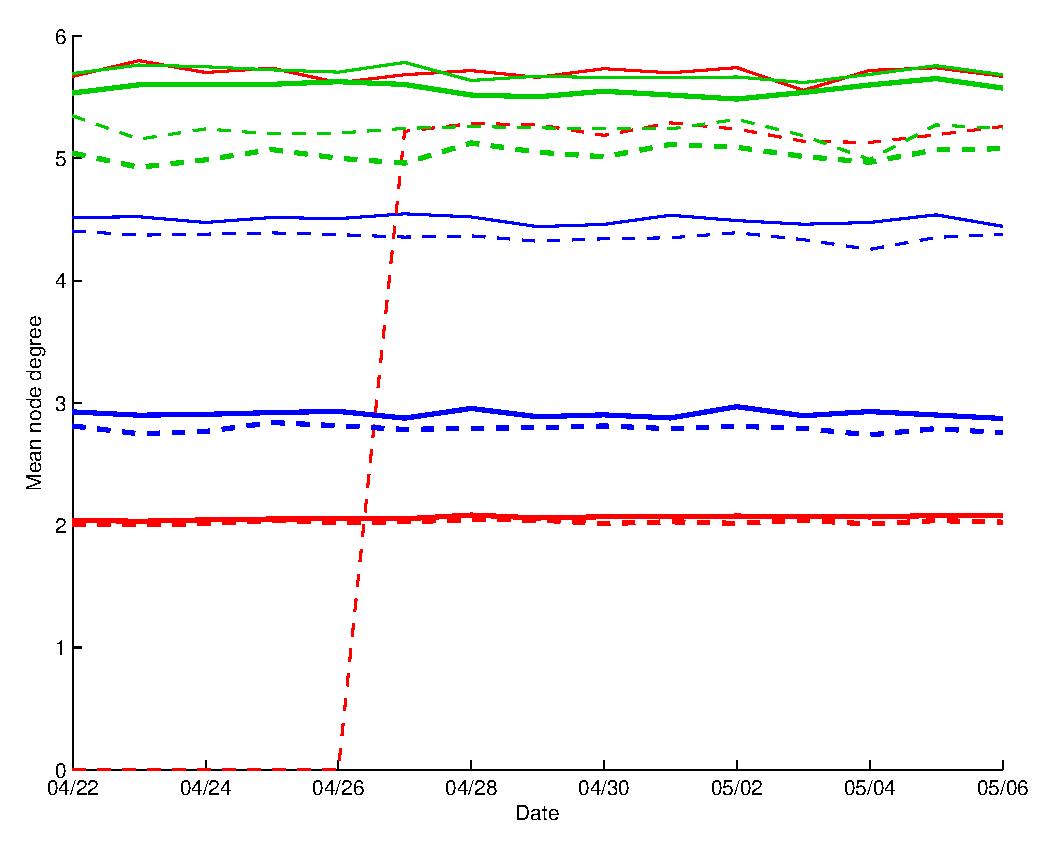
\includegraphics[width=.45\textwidth]{figures/plots/third-means.eps}\label{fig:third_means}} \hfill
  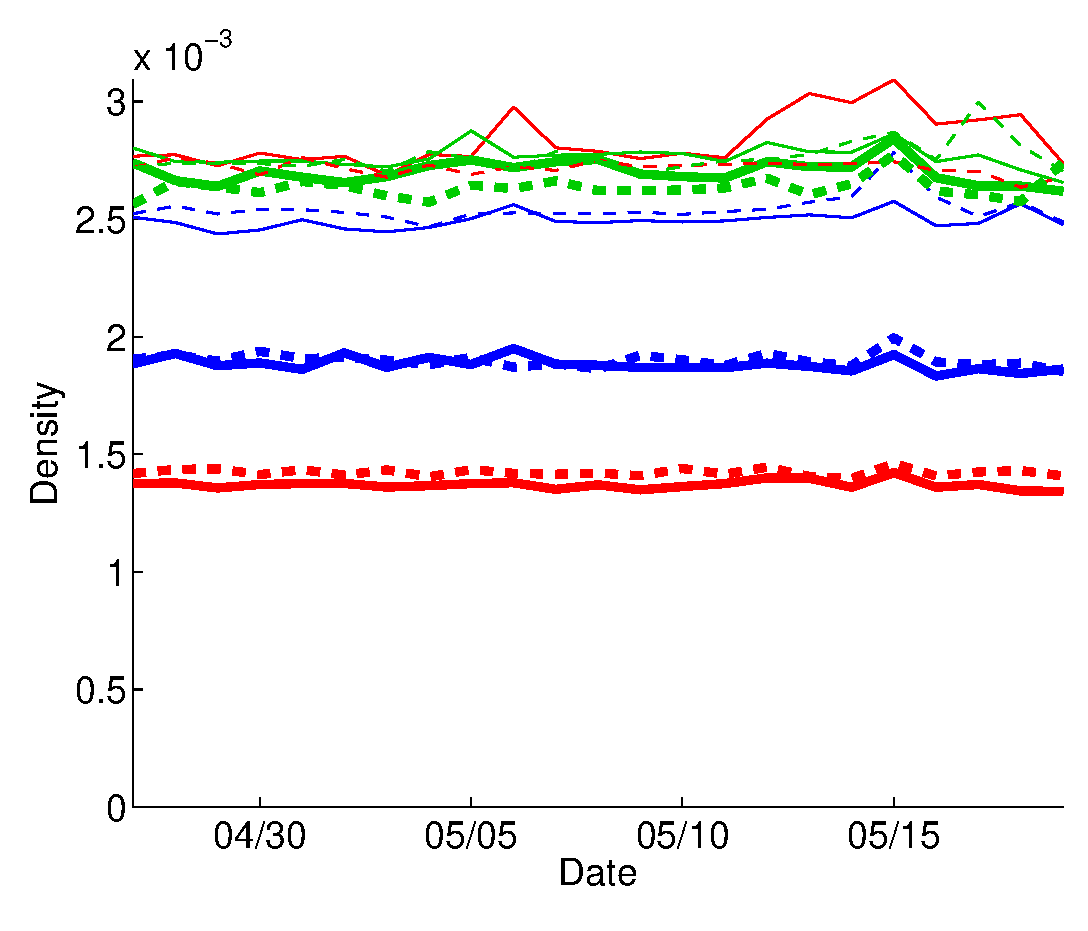
\includegraphics[width=.45\textwidth]{figures/plots/density.eps}

  \caption{Time evolution of the graph density for all browser profiles.}
  \label{fig:metrics_graphdensity}
  \end{figure}


As in Figure~\ref{fig:metrics_graphdensity}, grouping the TPD nodes according to the legal entities they belong to brings a considerable reduction of the mean FDP node degree, asserting that the number of legal entities potentially collecting information about the user is indeed less than that of the actual third-party domains tracking them.

On the contrary, the mean TPD node degree, as well as the graph density do not present any significant variation, which leads us to the conclusion that the various legal entities have on average access to roughly the same first parties, although controlling multiple third-party domains.



%In this section, we present our experimental results.
%In this subsection, we outline the experimental setup and configuration. To this end we make use of Lightbeam (a Firefox browser extention) in order to build the graph $G$.


%\subsubsection{Mean TPD node degree and graph density over time}
%We now study the evaluation of the TPD node degree and the graph density over time. Recall that the node degree of a TPD indicates how many of the FPDs this TPD has access to.

%We observe (Figure~\ref{fig:third_means}) that the browser profiles \textit{Ghostery\_Default} and \textit{NoAdblocker} have the worst filtering performance, since the third parties loaded have access to the highest mean number of first parties. Although we would expect that the use of an adblocker, such as Ghostery, should provide us with better results, a closer look at its initial settings shows that the adblocker functions as a third-party tracker that does not block any third parties by default, unless configured appropriately. The metric has a consistently but only slightly lower value for the profile \textit{NoAdblocker\_DNT}.

%The browser profiles with the same settings but with a Mobile User Agent (\textit{Ghostery\_\allowbreak Default\_\allowbreak MUA}, \textit{NoAdblocker\_\allowbreak MUA} and \textit{NoAdblocker\_\allowbreak DNT\_\allowbreak MUA}) have a mean TPD node degree lower by roughly 15\%. Comparing the three browser profiles with each other though, we see that their relative order remains unaltered.

%AdblockPlus (\textit{Adblockplus\_\allowbreak Default} and \textit{Adblockplus\_\allowbreak Default\_\allowbreak MUA}) with its default settings has a mean TPD node degree significantly lower than the aforementioned worst cases, i.e. no adblocker or Ghostery at its default configuration.

%Unsurprisingly, the browser profiles that filter the most third parties are those configured to a maximum protection level. We observe that the mean node degree decreases by approximately 80\% compared to the default protection level. Ghostery moreover consistently performs better than AdblockPlus, when both are set to the maximum protection settings.

%An inspection of the graph-density plot (Figure~\ref{fig:density}) for each of the profiles tested yields similar results: The profiles \textit{Ghostery\_\allowbreak Default} and \textit{NoAdblocker} present the worst filtering efficiency, setting the DNT header brings a slight amelioration, the usage of AdblockPlus even with default settings comes with considerably better results, whilst the best filtering performance is achieved by the profile \textit{Ghostery\_\allowbreak MaxProtection} followed by \textit{Adblockplus\_\allowbreak MaxProtection}. Nonetheless, the use of Mobile User Agent seems now to deteriorate the graph density, although it improved the TPD node degree. We explain this behavior with the fact that from all of the third parties that were loaded under a Desktop User Agent, only the most popular ones are still loaded under a Mobile User Agent, i.e.\ the ones that have a higher chance of being requested by more FPDs, e.g. \texttt{doubleclick.net}. Henceforth, although the mean TPD node degree is lower for the Mobile User Agent, the absolute number of TPD nodes is also considerably lower compared to the Desktop User Agent, which leads to a higher graph density according to Formula~\ref{eq:density}, or equivalently a more connected graph.

%Because, the User Agent however is not a privacy-related setting ---e.g. adblocker, protection level, DNT header--- the analysis of the filtering performance of a configuration does not involve the impact of this parameter on the achieved privacy level. As a consequence, the graph density still provides a valid metric for the evaluation and comparison of the filtering effectiveness of different privacy configurations.

 % \begin{figure*}[!t]
 %  \centering
% \subfloat[Mean value of the degree of the FPD nodes over time for each browser profile $U$]{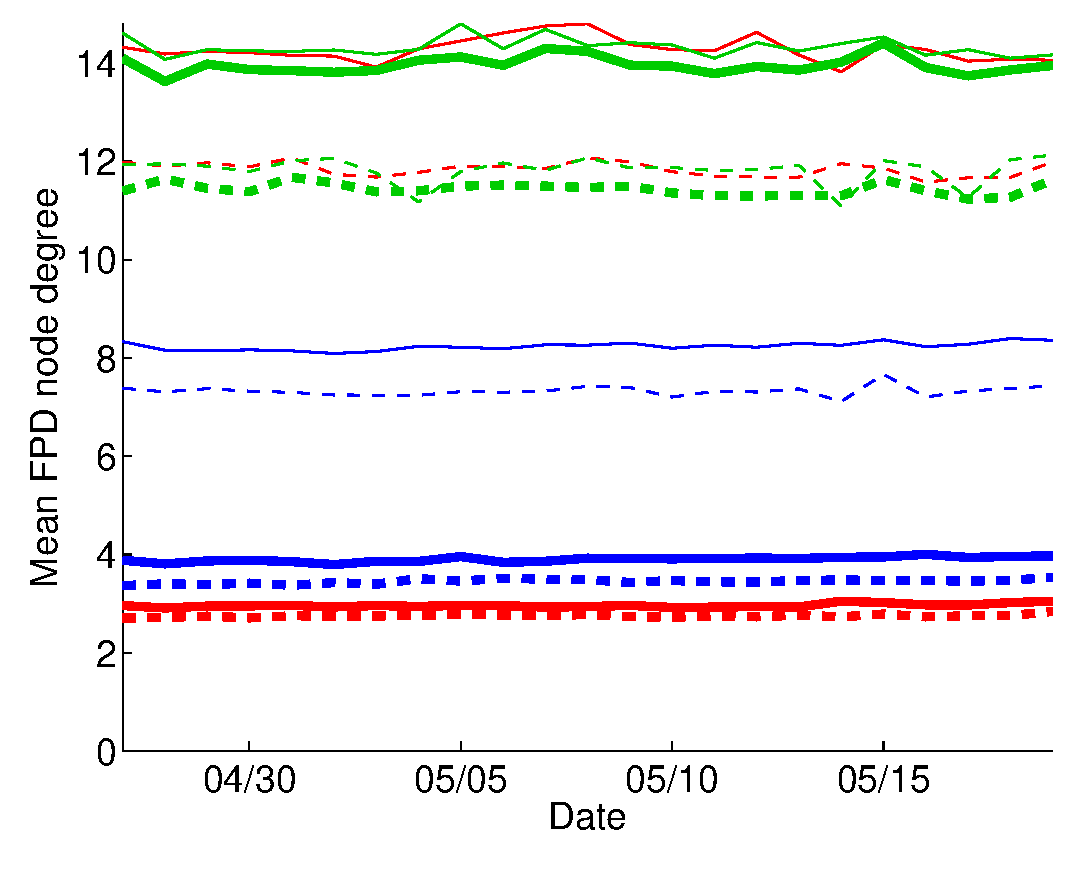
\includegraphics[width=.45\textwidth]{figures/plots/first-means.eps}\label{fig:first_means}}
%  \subfloat[Mean TPD node degree]{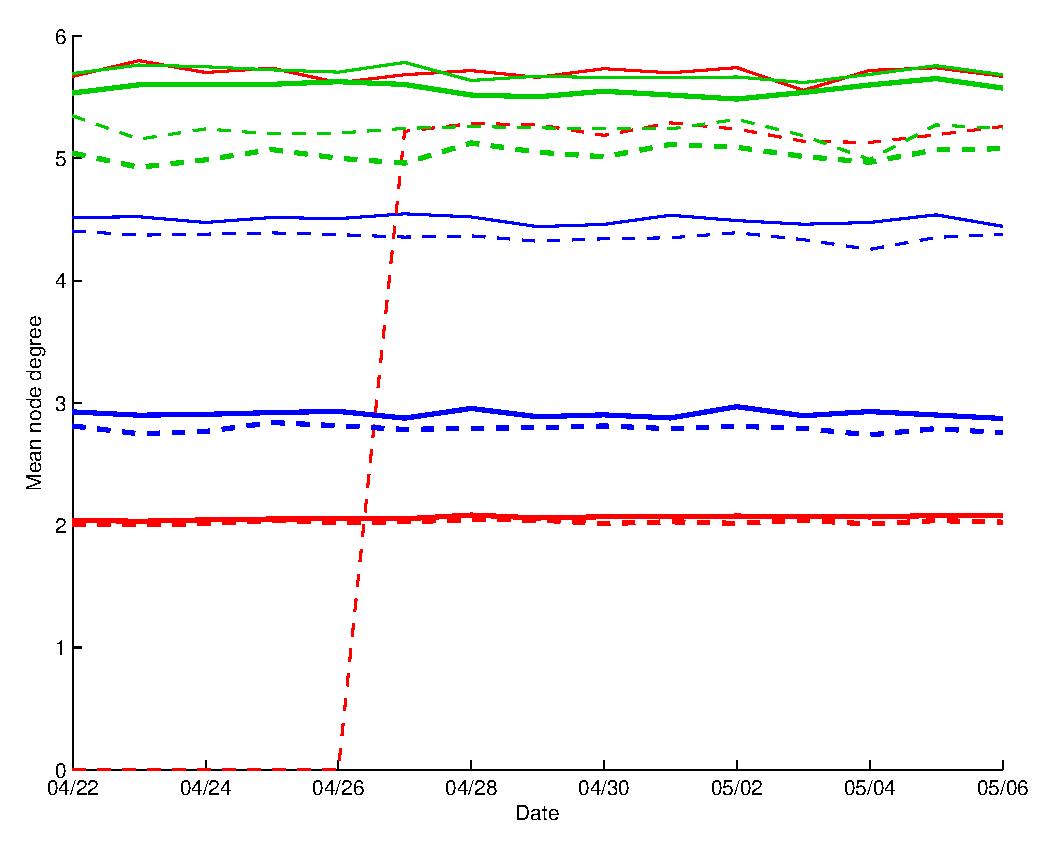
\includegraphics[width=.45\textwidth]{figures/plots/third-means.eps}\label{fig:third_means}} \hfill
%  \subfloat[Graph density]{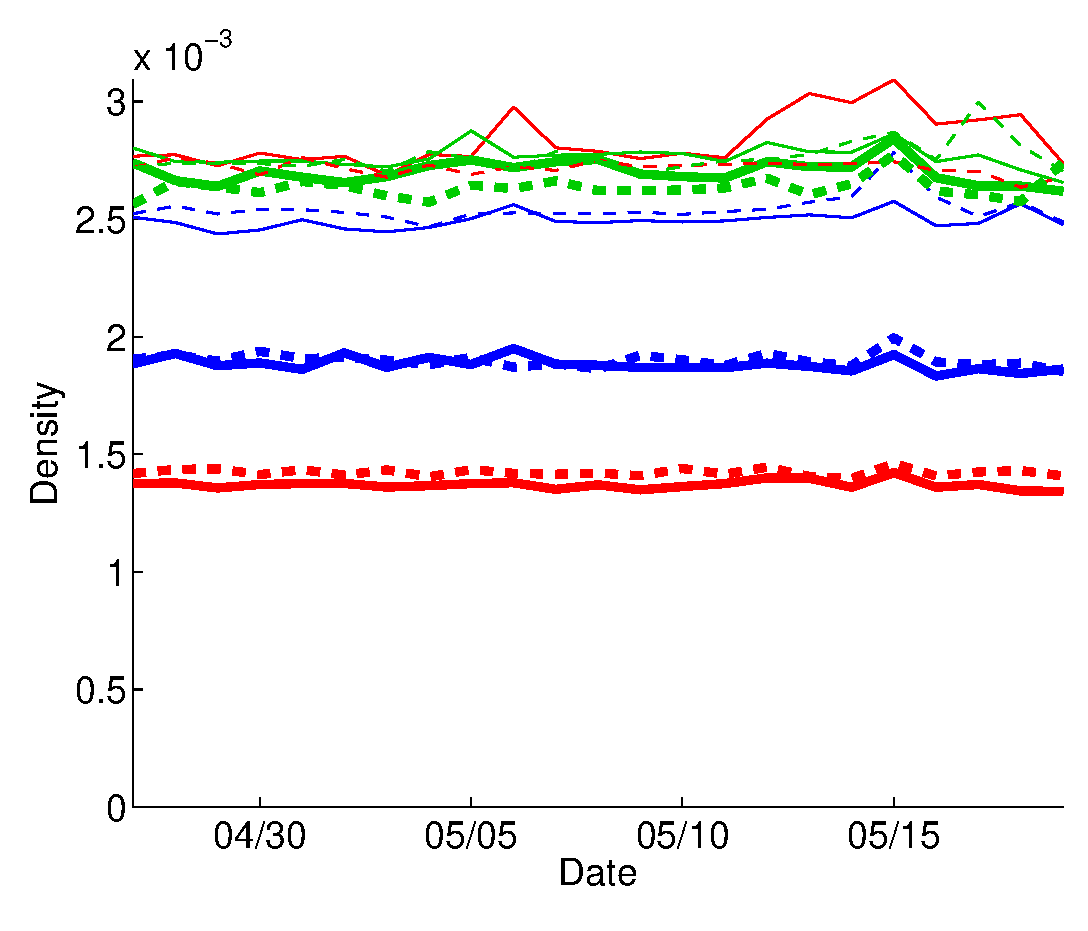
\includegraphics[width=.45\textwidth]{figures/plots/density.eps}\label{fig:density}}

 % \caption{Time evolution of mean TPD node degree and graph density for all browser profiles}
 % \label{fig:metrics_without_entities}
 % \end{figure*}


%\begin{figure*}[!t]
%  \centering
%  \subfloat[FPD node degree]{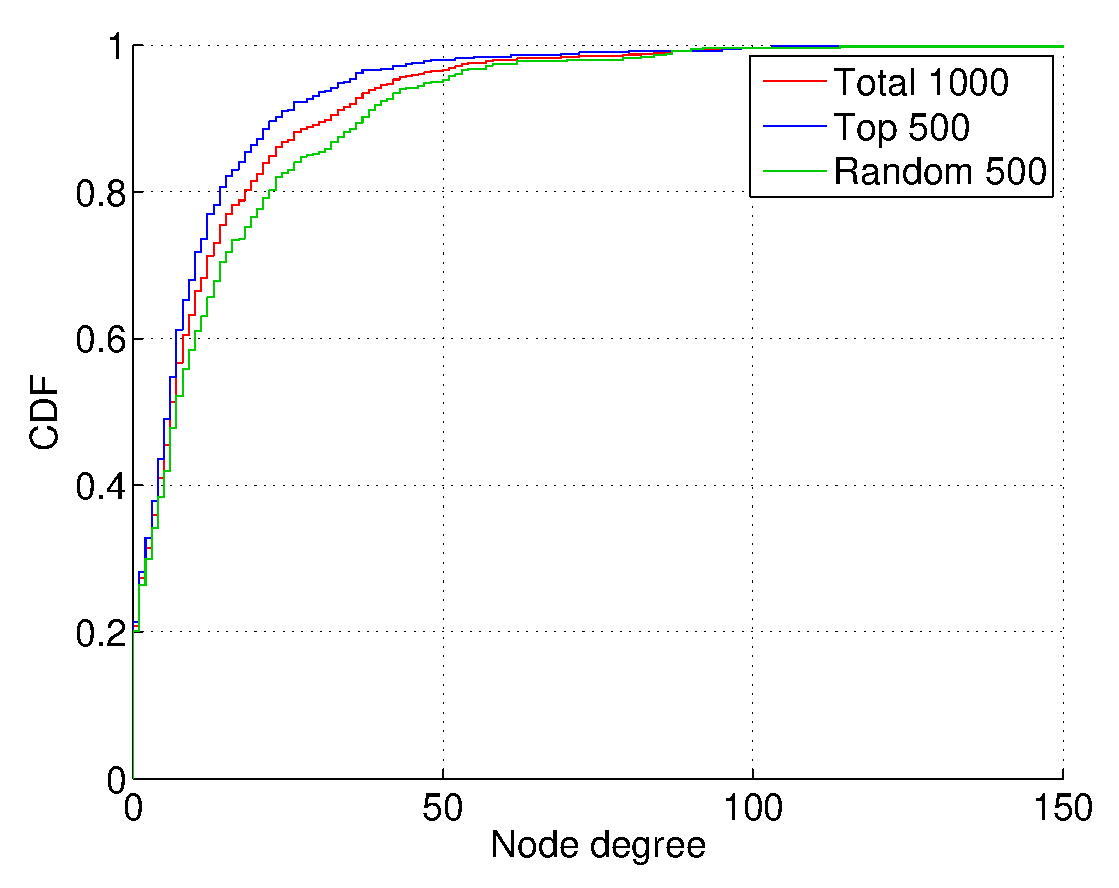
\includegraphics[width=.45\textwidth]{figures/plots/cdf-first-node-degree.eps}\label{fig:cdf-first-node-degree}} %\hfill
%  \subfloat[TPD node degree]{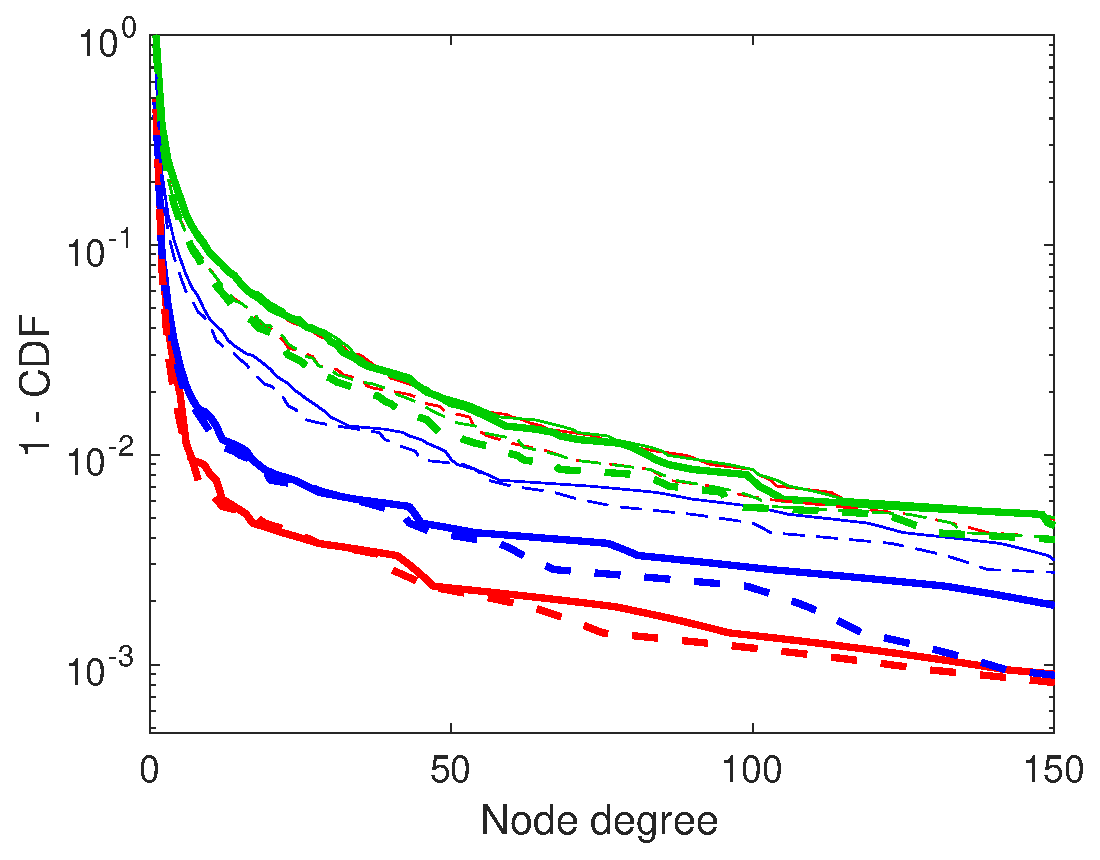
\includegraphics[width=.45\textwidth]{figures/plots/cdf-third-node-degree.eps}\label{fig:cdf-third-node-degree}}

%    \caption{CDF of FPD and TPD node degree for all browser profiles on 27/04/2016}
%    \label{fig:cdf_first_third_node_degree}
%\end{figure*}

%\subsubsection{Graph separation}
% \textbf{Graph separation (Figure~\ref{fig:top_last_domains_comparison}):}
%In order to investigate whether the ad-blocking tools have been subject to optimizations that would enable better filtering performances for the top-visited domains, our URL sample set $W$ includes, as explained in Section~\ref{sec:crawled_urls}, an additional set of 500 domains with a rank uniformly selected between 500 - 1M from the Alexa Top Rank. To this end, we separate the original graph $G$ into two independent graphs $G_T$ and $G_R$ for the 500 top-visited and the 500 uniformly-selected URLs, respectively, and followingly directly compare their filtering performances.

%Figure~\ref{fig:top_last_domains_comparison} provides a comparison of the ad-blocking efficiency of the browser profiles $U$ for the two URL subsets. We observe that, the filtering performance of the different profiles remains roughly unaffected. We observe that Ghostery and AdblockPlus reduce the FPD node degree by an approximate factor of 5.7 and 4.3 for the top 500, while only 3.7 and 3 for the uniformly-selected 500 websites.

%On one hand, this indicates a better filtering performance of Ghostery and AdblockPlus for the 500 top-ranked websites compared to the 500 uniformly-selected ones. On the other hand, Figure~\ref{fig:top_last_domains_comparison} shows that the mean FPD node degree of the 500 top-ranked websites (\textasciitilde17) is consistently and clearly higher than that of the 500 uniformly-selected websites (\textasciitilde12) without the use of any adblocker (profile \textit{NoAdblocker}). The 500 top-ranked websites therefore provide a larger margin for TPD node degree reduction or, equivalently, a bigger opportunity for improvement in terms of privacy. %To illustrate, supposed that a powerful adblocker could block all TPDs, its eventually measured filtering performance would be considerably higher for the 500 top-ranked URLs than for the 500 uniformly-selected ones.

%Although an rank-oriented optimization of the adblockers seems plausible at a first glance, the different margins of improvement for the 500 top-ranked and the 500 uniformly-selected URLs do not allow us to judge whether adblockers are optimized for the top 500 websites or not.







%\subsubsection{Highest-degree domains}
%In this section we focus particularly on the first parties that load the highest number of third parties. To this end, we evaluate on a daily basis the top 1 (Figures~\ref{fig:first_mean_top1_without_entities},~\ref{fig:third_mean_top1_without_entities}) and top 10 domains (Figures~\ref{fig:first_mean_top10_without_entities},~\ref{fig:third_mean_top10_without_entities}) that load most third parties.

%After an examination of the Figure~\ref{fig:highest_degree_nodes}, we observe that in the worst case, a first-party website can be tracked by up to 170 third parties (Figure~\ref{fig:first_mean_top1_without_entities}), while a third-party can have access and collect information about our browsing behavior from almost 500 first-party websites that we visited (Figure~\ref{fig:third_mean_top1_without_entities}). It is, however, important to mention that the filtering performances of the browser profiles $U$ remain approximately in the same relative order as in the previously analyzed cases, with the use of the adblockers to considerably enhance the user's protection against tracking. We observe naturally that the results present higher variations than when averaging 1000 websites.


 %   \begin{figure*}
 %  \centering

 %  \subfloat[Highest degree of FPD nodes for each day and browser profile $U$]{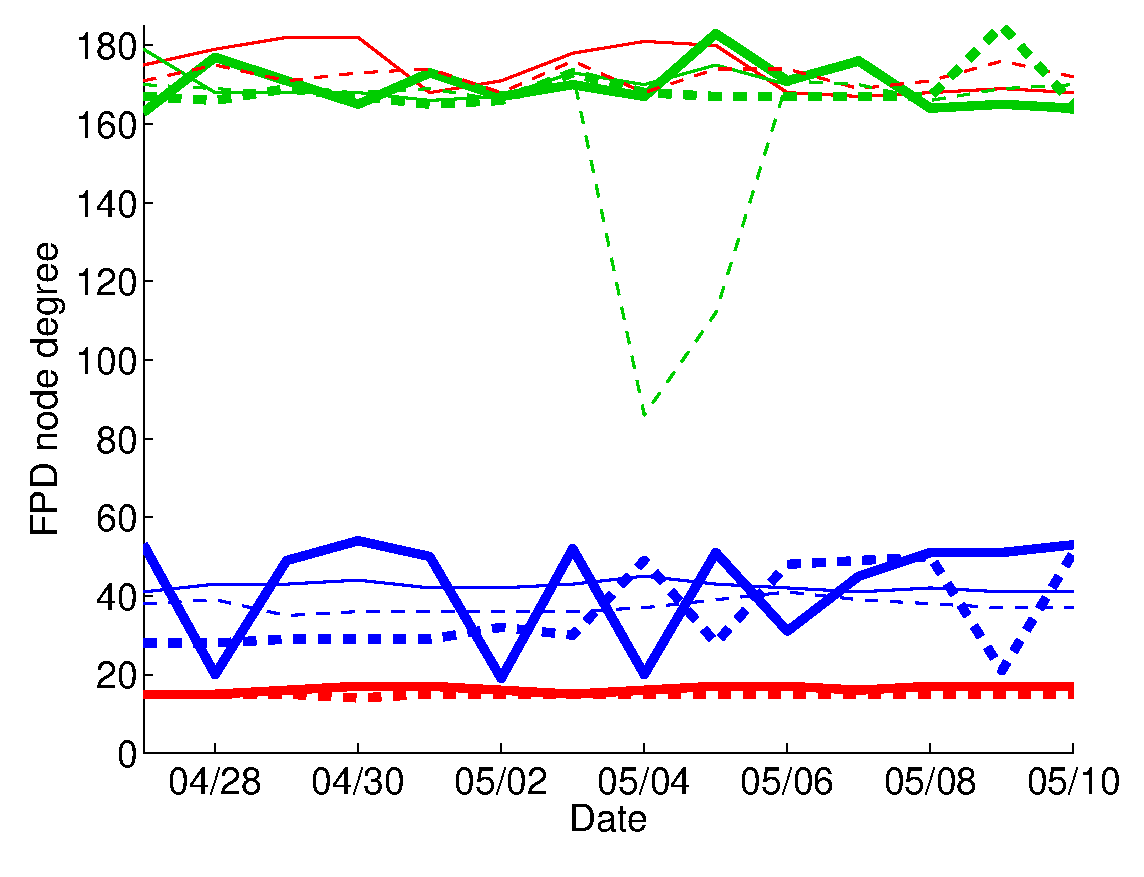
\includegraphics[width=.45\textwidth]{figures/plots/first-mean-top1.eps}\label{fig:first_mean_top1_without_entities}} \hfill
 %  \subfloat[Mean value of the degree of the 10 most-connected FPD nodes for each day and browser profile $U$]{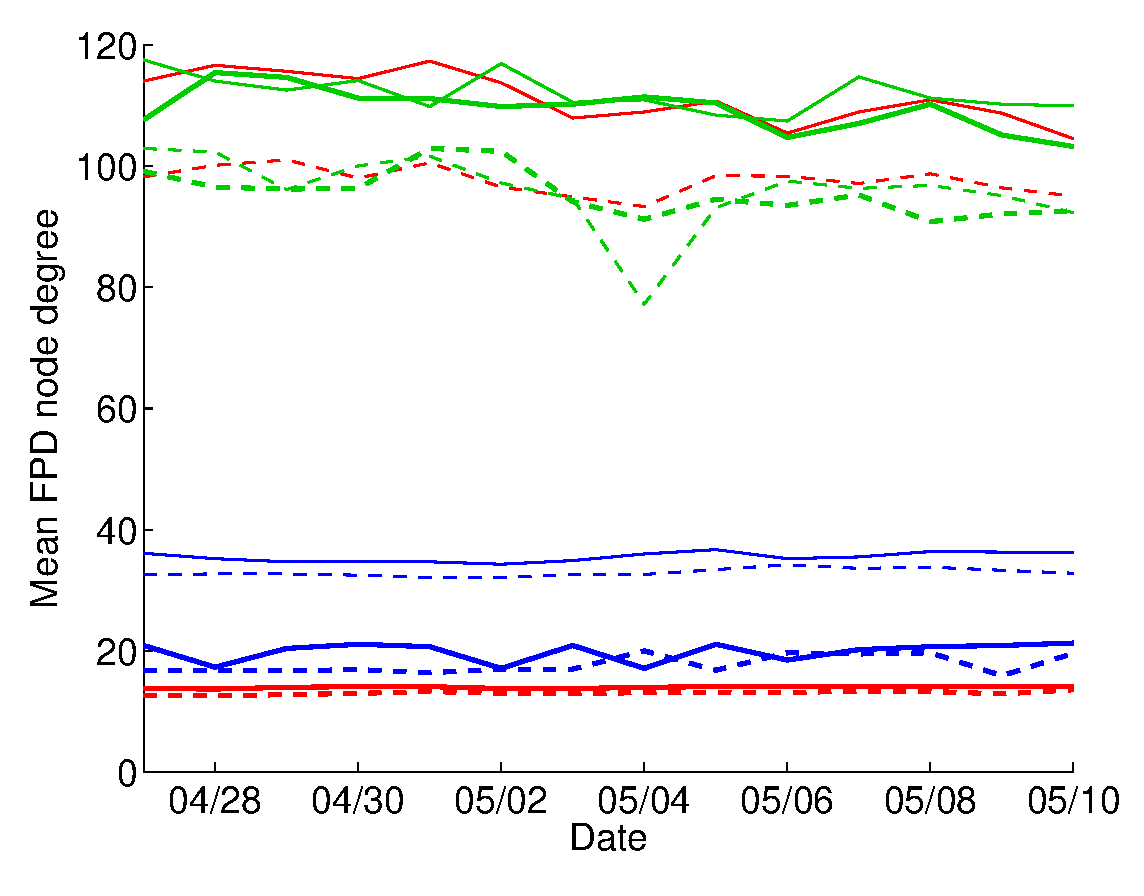
\includegraphics[width=.45\textwidth]{figures/plots/first-mean-top10.eps}\label{fig:first_mean_top10_without_entities}} \\
 %  \subfloat[Highest degree of TPD nodes for each day and browser profile $U$]{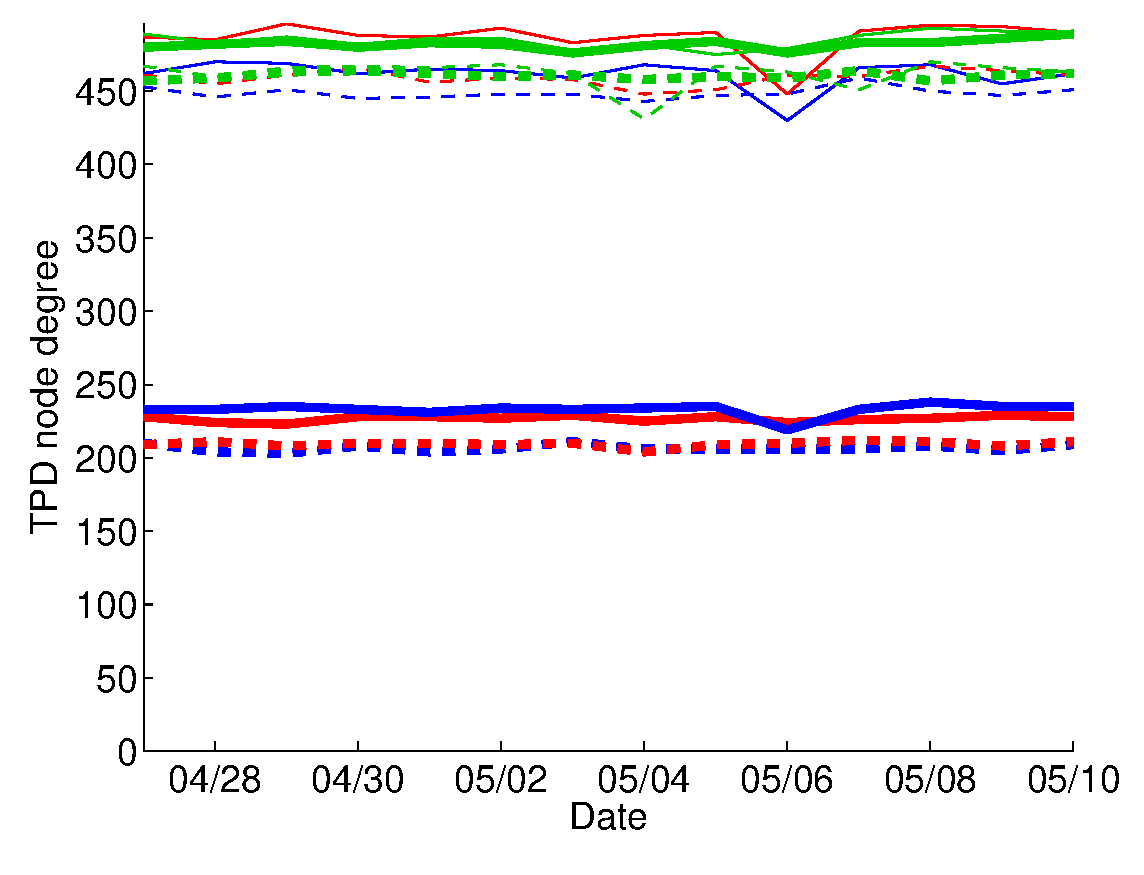
\includegraphics[width=.45\textwidth]{figures/plots/third-mean-top1.eps}\label{fig:third_mean_top1_without_entities}} \hfill
 %  \subfloat[Mean value of the degree of the 10 most-connected TPD nodes for each day and browser profile $U$]{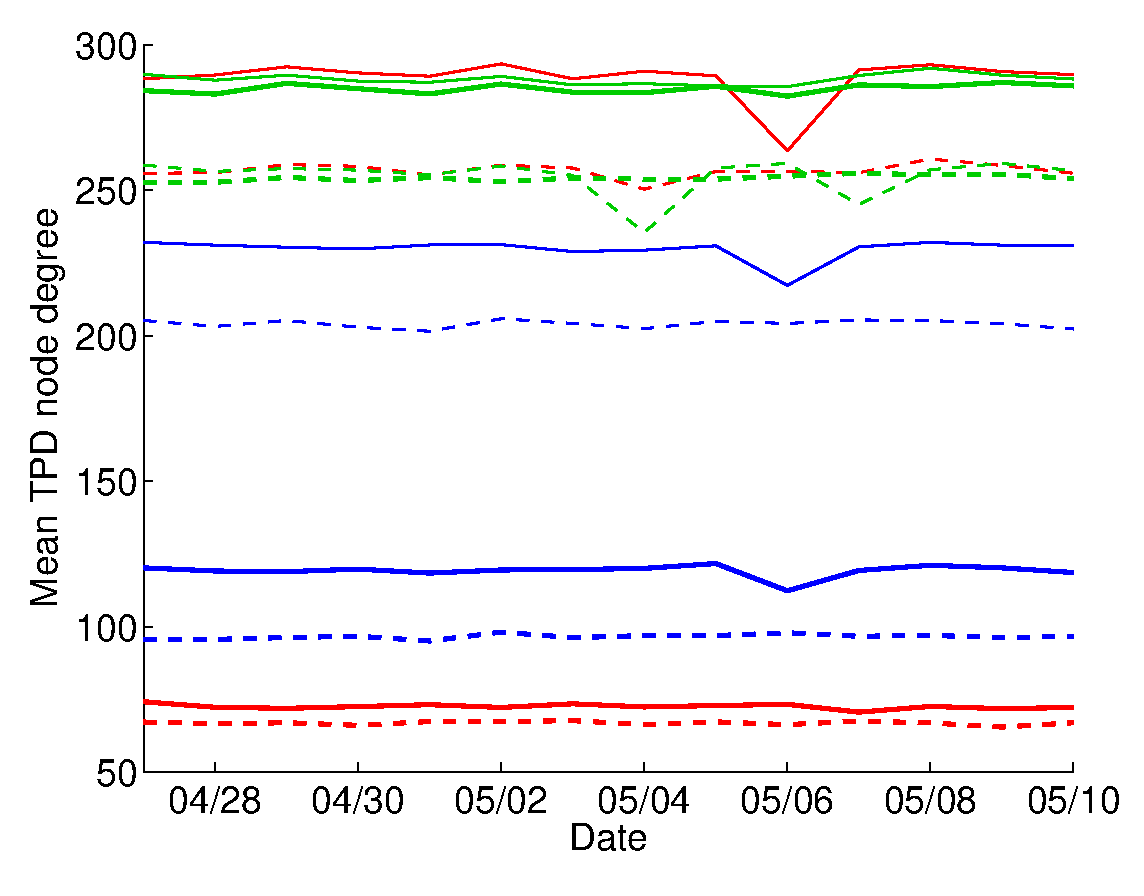
\includegraphics[width=.45\textwidth]{figures/plots/third-mean-top10.eps}\label{fig:third_mean_top10_without_entities}}

 % \caption{Time evolution of the first and third-party degree metrics for the most-connected FPD and TPD nodes, respectively}
 % \label{fig:highest_degree_nodes}

 % \end{figure*}

% \begin{figure}
%  \centering
%  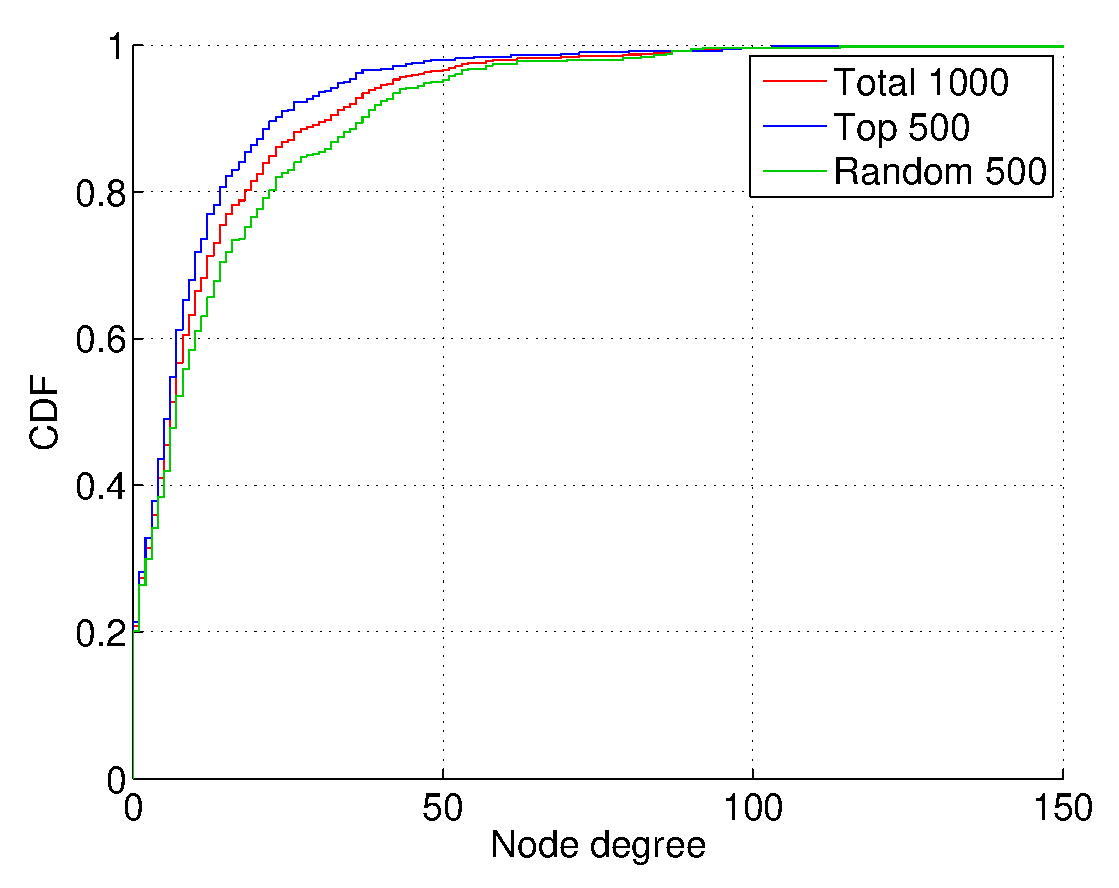
\includegraphics[width=.45\textwidth]{figures/plots/cdf-first-node-degree.eps}
%  \caption{Cumulative distribution function of FPD node degree for the browser profile \textit{NoAdblocker} on 28/04/2016}
%  \label{fig:cdf_first_node_degree}
% \end{figure}




%\subsubsection{Metrics with entity grouping}
%We now build the graphs $G_E$ that correspond to each browser profile $U$ by grouping multiple TPD nodes into one supernode representing their common administrative organization (legal entity) as described in Section~\ref{sec:legal_entity} and visualized in Figure~\ref{fig:graph}. We refer to this supernode as \textit{third-party entity} (TPE). Note that the FPDs remain unaltered in the new augmented graph. When we observe TPEs instead of TPDs, the mean FPD node degree is on the one hand reduced as an absolute number, while on the other hand, no considerable changes are to be observed for the mean TPE node degree or the graph density. As far as the relative ad-blocking efficiency of the browser profiles is concerned, we should remark that this does not present any change with respect to the results before entity grouping had been applied.

%Comparing the mean FPD node degrees over time for the graphs $G$ (without entity grouping) and $G_E$ (with entity grouping) we observe that each visited URL from the sample set $U$ loads approximately 14 TPDs, but 12 TPEs on average. From graph $G$ we see that using AdblockPlus and Ghostery with maximal-protection configurations reduces the mean number of TPDs loaded by about 3.5 and 4.7 times, accordingly. Similarly, according to graph $G_E$, AdblockPlus and Ghostery reduce the mean number of TPEs loaded by roughly 3.4 and 4.8 times, respectively.

% \begin{figure}[!t]
%   \begin{subfigure}{.45\textwidth}
%     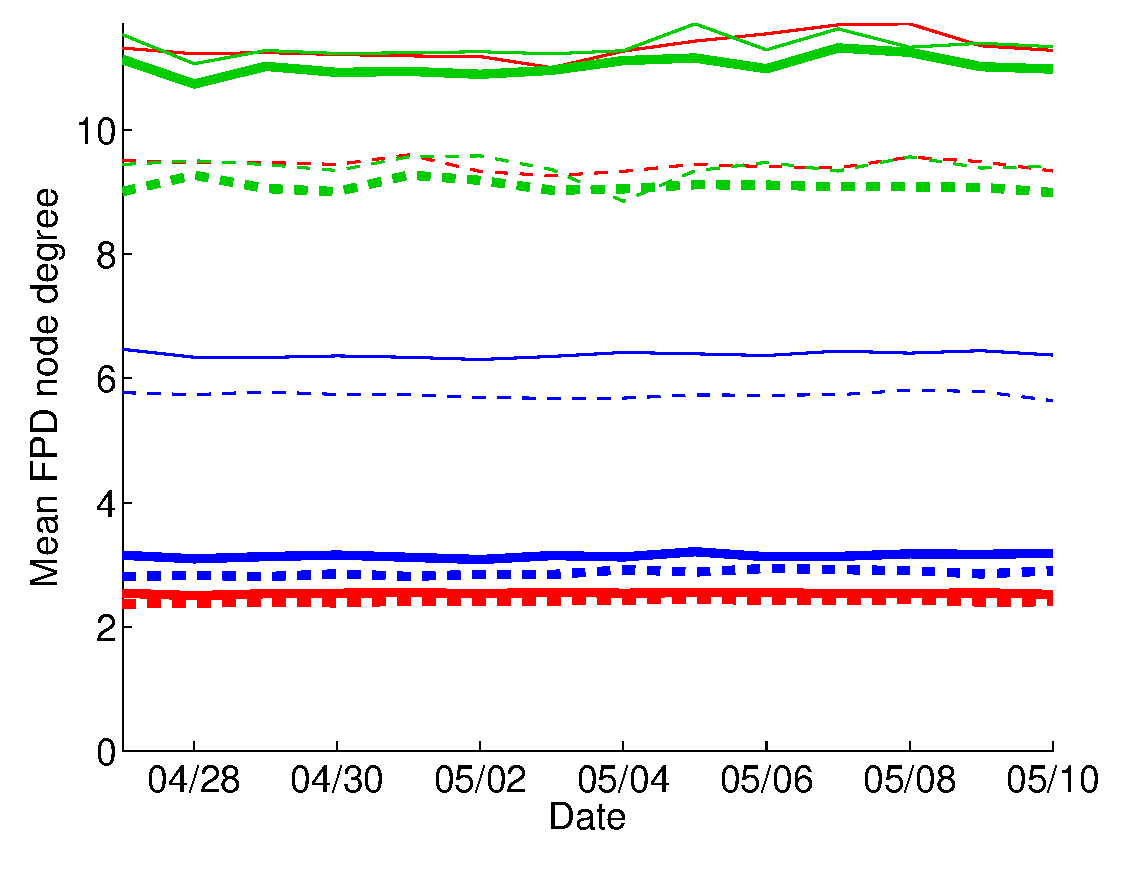
\includegraphics[width=\textwidth]{figures/plots/first-means-entities.eps}
%     \caption{Mean value of the degree of the FPD nodes over time for each browser profile $U$}
%     \label{fig:first_means_entities}
%   \end{subfigure}

%   \begin{subfigure}{.45\textwidth}
%     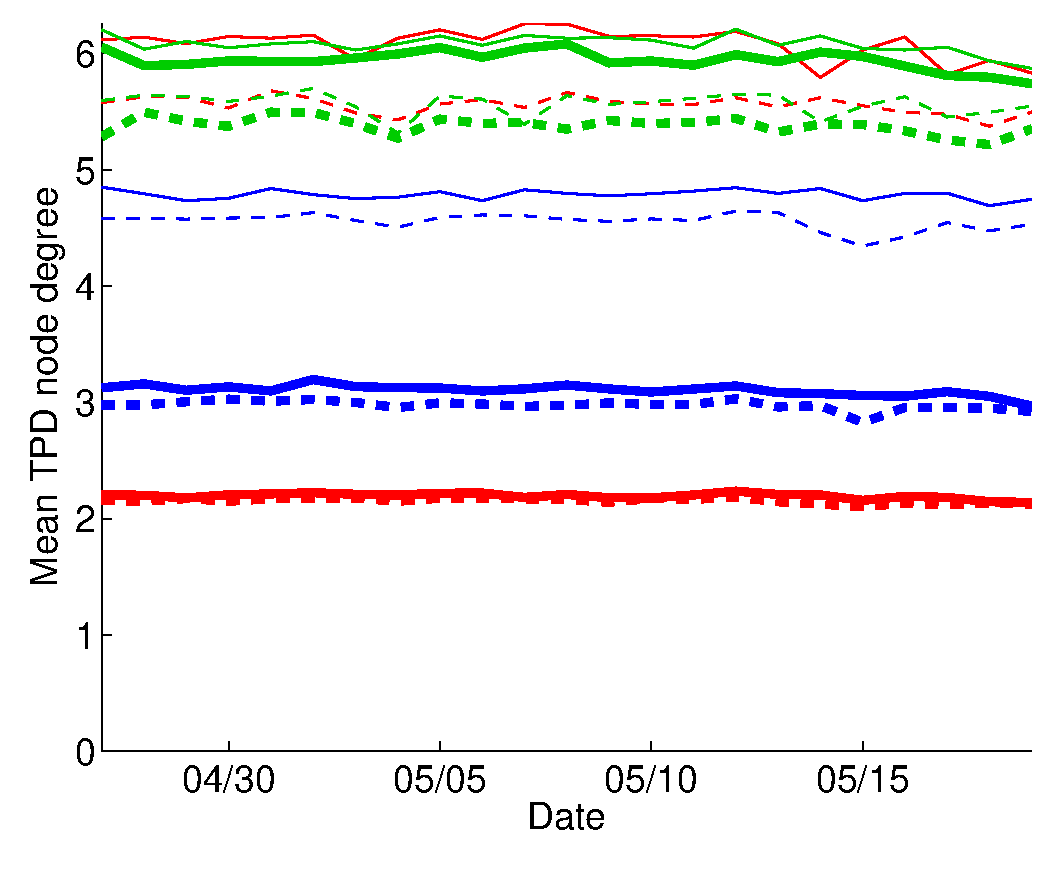
\includegraphics[width=\textwidth]{figures/plots/third-means-entities.eps}
%     \caption{Mean value of the degree of the TPD nodes over time for each browser profile $U$}
%     \label{fig:third_means_entities}
%   \end{subfigure}

%   \begin{subfigure}{.45\textwidth}
%     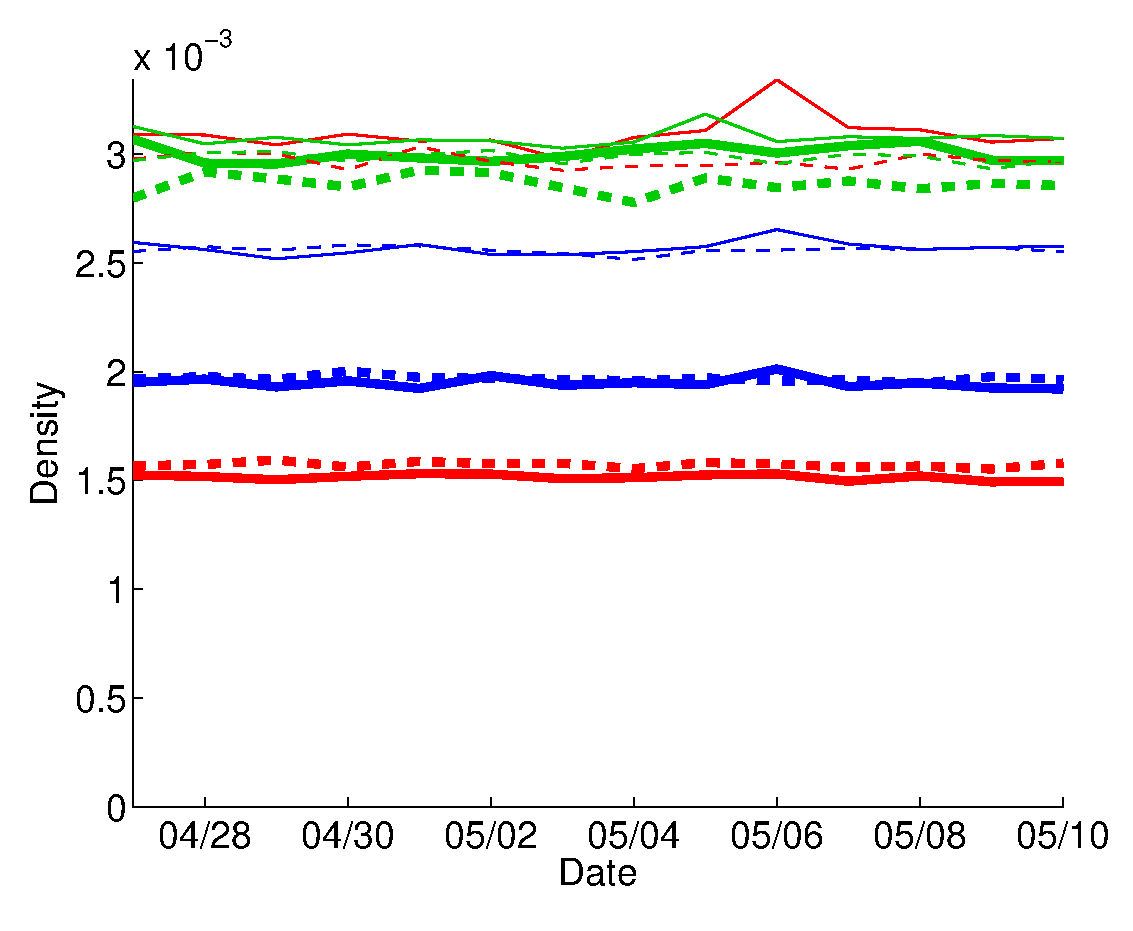
\includegraphics[width=\textwidth]{figures/plots/density-entities.eps}
%     \caption{Density of graph $G$ over time for each browser profile $U$}
%     \label{fig:density_entities}
%   \end{subfigure}
%   \caption{Time evolution of the metrics \textbf{with} domain grouping according to entities. {\color{red}Remove Figure and add text on how much the y-axis changes when you do domain grouping.}}
%   \label{fig:metrics_with_entities}
%   \end{figure}

% \subsubsection{Metric intuition}
% Notwithstanding that the relative filtering performance of the browser profiles remained practically unaltered with the use of the different metrics, as illustrated above, the discrepancies between the results of the profiles are not always trivial to tell apart. As a consequence, the mean TPD node degree is less suitable than the mean FPD node degree when profiles with smaller efficiency differences are to be discerned, while their distignuishability weakens markedly further when the graph density is used as a metric.


\section{Discussion}
This section summarizes our findings and discusses the influence of profile parameters on the user privacy:
%As explained in Section~\ref{sec:browser_profiles}, the browser profiles $U$ are created as a combination of different profile parameters under inspection. After a thorough examination of the experimental results of the previous sections, the impact of these parameters can be summarized as follows:

\vspace{0.5 em}\noindent \textbf{Adblocker installed:} Our results show that the use of an adblocker significantly reduces the number of third parties loaded by a factor of 40\% for an adblocker with default settings. By default Ghostery does not function as adblocker, while with maximum protection, Ghostery consistently outperforms AdblockPlus.

\vspace{0.5 em}\noindent \textbf{Block policy:} The block policy configured ---i.e. default or maximum protection--- for each adblocker results in a blocking difference of almost 80\% and 50\% for the mean first-party degree for Ghostery and AdblockPlus, respectively.

\vspace{0.5 em}\noindent \textbf{Do Not Track header:} The activation of the DNT flag has little impact on the results, since the browser user has no control over whether the DNT flag is honored or not and hence websites and advertisers may either obey or completely ignore~it.

\vspace{0.5 em}\noindent \textbf{Mobile User Agent:} Websites that received requests by a mobile user agent indeed responded with a considerably lower number of third parties. A plausible explanation for this behavior is the requirement for less bandwidth that the mobile websites usually conform to. As a consequence of this limitation, less content is loaded and hence less requests are sent to third parties. This discrepancy was of course less obvious for the browser profiles with maximal protection enabled, since tracking by third parties is already reduced. To exemplify, in Figure~\ref{fig:top500_first_means} the profiles \textit{Ghostery\_Default}, \textit{NoAdblocker} and \textit{NoAdblocker\_DNT} present a mean FPD node degree about 20\% higher than the corresponding browser profiles where a Mobile User Agent is used.

\vspace{0.5 em}\noindent \textbf{Tracking:}
A few legal entities such as Google and Facebook are able to track users across many first-parties (67\% for Google and 33\% for Facebook). In their maximum protection level, adblockers such as Ghostery and Adblock Plus are able to suppress effectively third-party requests to these legal entities. However legal entities such as Google that host content (e.g., libraries) in addition to advertisements are still able to track visits to more than 30 \% of the first parties.

\vspace{0.5 em}\noindent \textbf{Geographical distribution:}
While some countries host proportionally more third-parties than first parties such as the United States and China, adblockers tend to reduce the number of third-party requests equally well irrespective of the origin country.

\vspace{0.5 em}\noindent \textbf{Temporal dynamics:} In general, the privacy of users is not very sensitive to web site or blacklist optimizations that happen at shorter time scales. However, some few domains exhibit larger temporal variations of the amount of third-party requests by more than 50~percent, suggesting that these sites may perform optimizations on their domains to reduce the impact of adblockers.
% \begin{figure}
%  \centering
%  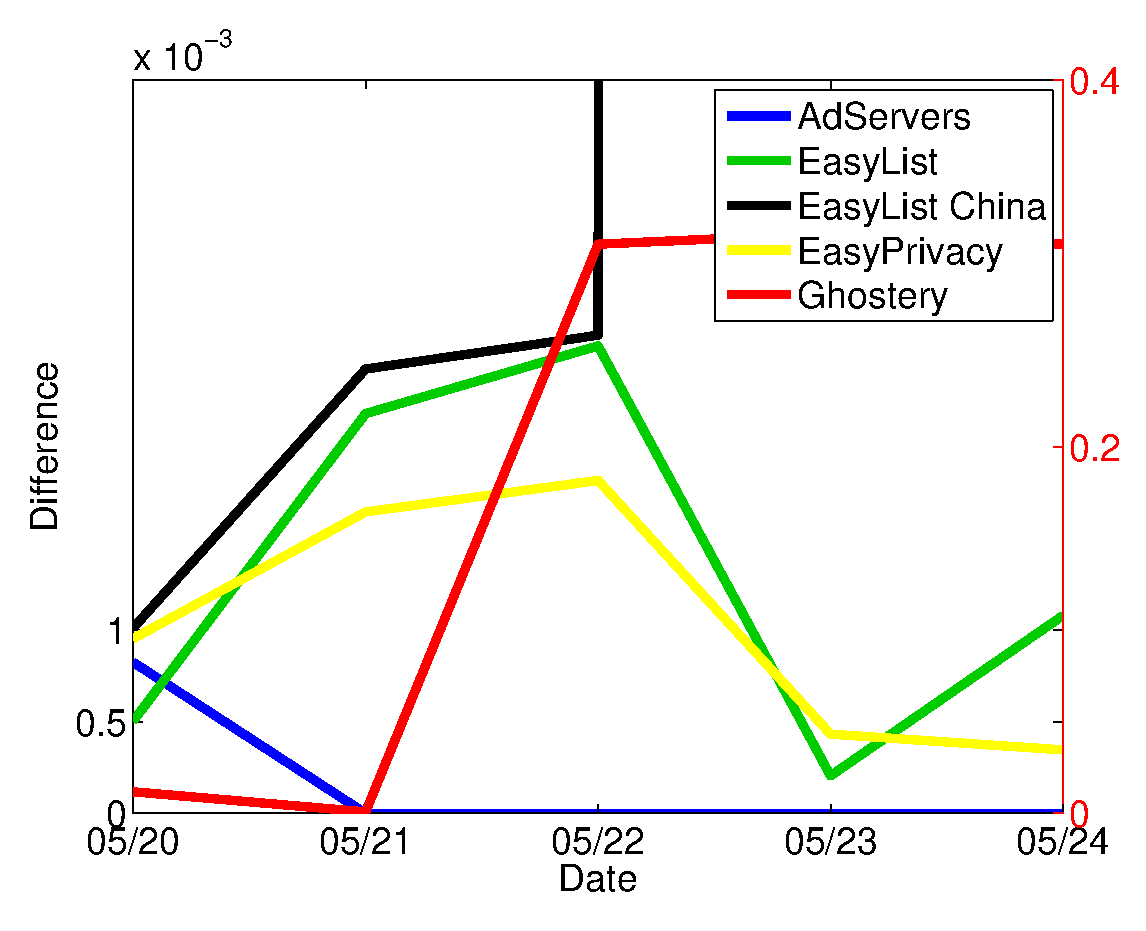
\includegraphics[width=.45\textwidth]{figures/plots/blacklist-diff.eps}
%  \caption{Difference between a blacklist and its version on the previous day}
%  \label{fig:blacklist-diff}
% \end{figure}





%\subsection{Rank impact}

%In Figures~\ref{fig:top_last_domains_comparison} and~\ref{fig:cdf_first_node_degree} we investigated the relationship between the URL rank and the FPD node degree. As resulted from the plot of the mean FPD node degree, the uniformly-selected FPD nodes were accessed on average by less third parties with respect to the top-ranked 500 FPD nodes, thus contradicting our initial assumption. On the other hand, a higher number of loaded third parties can be justified, if the size and the popularity of the first domains is taken into consideration, as opposed to that of the last domains.

%Another observation can be made when the correlation between the rank and the FPD node degree is examined. More specifically, the rank of each website among the top 500 of the rank (Figure~\ref{fig:first_party_degree_relative_rank}) does not present a strong correlation to the number of third parties it loaded, hence reinforcing our conclusion above.

\section{Related work}
\label{sec:related_work}

%HOW TRACKING CAN BE DONE??? (http://download.springer.com/static/pdf/160/chp%253A10.1007%252F978-3-319-17172-2_8.pdf?originUrl=http%3A%2F%2Flink.springer.com%2Fchapter%2F10.1007%2F978-3-319-17172-2_8&token2=exp=1464349113~acl=%2Fstatic%2Fpdf%2F160%2Fchp%25253A10.1007%25252F978-3-319-17172-2_8.pdf%3ForiginUrl%3Dhttp%253A%252F%252Flink.springer.com%252Fchapter%252F10.1007%252F978-3-319-17172-2_8*~hmac=d4b6217fa9f198f9101de1917e7f672f2f37025beb9eefe3ac7654778a2954c3)

\textbf{Privacy concerns:} Many works in the literature have been dedicated to the privacy concerns as a consequence of tracking and fingerprinting by third-party domains~\cite{barford, englehardt, krishnamurthy_privacy_diffusion, nikiforakis, soltani, libert2015exposing}. Castelluccia \textit{et al.}~\cite{castelluccia} showed that the user's interests can be inferred by the ads they receive and their whole profile can be reconstructed. This can lead to discriminations of the users according to their profile details and configurations, as shown in~\cite{mikians, datta}.

\textbf{Countermeasures:} As a result, several methods have been proposed that enable targeted advertisements without compromising user privacy~\cite{adnostic, privad, nurikabe, haddadi, juels, androulaki}. Additionally, there have been a lot of attempts for the detection of tracking behavior and ad-blocking blacklist ehnancements~\cite{ma, gugelmann, tran}, while some studies have proposed further mitigation techniques~\cite{roesner, kontaxis}.

\textbf{Comparison of mitigation-techniques:} Since our work focuses on the comparison of the ad-blocking tools, it is useful to present in more detail the work done so far in this field.

Balebako \textit{et al.}~\cite{balebako} propose a method to measure behavioral targeting and the effect of privacy-protection techniques ---e.g. disabling of third-party cookies, Do-Not-Track header, ad-blocking tools--- in the limitation of the behavioral-targeted character of the advertising content, while Krishnamurthy \textit{et al.}~\cite{krishnamurthy_measuring_privacy_loss} compare different privacy-protection techniques against the trade-offs between privacy and page quality. Leon \textit{et al.}~\cite{leon} investigate and compare the usability of some existing tools designed to limit advertising.

Pujol \textit{et al.}~\cite{pujol} aim to infer the use or no use of an adblocker by examining the HTTP(S) requests sent by a browser, using the ratio of the ad requests and the downloads of filter lists as indicators. Moreover, the filtering performance of 7 different browser profiles ---adblocker-configuration combinations--- is compared based upon the total number of unblocked requests per browser profile. Furthermore, the ad traffic is examined and classified through the analysis of the number of requests at different time instances throught the day, the content-type of the ad requests, as well as the effect of enabling non-intrusive ads. However, the relationship between the first-party and third-party domains is not examined and no long-term data is collected regarding the tracking behavior of the third parties.

Ruffell \textit{et al.}~\cite{ruffel2015} analyze the effectiveness of various browser add-ons in mitigating and protecting users from third-party tracking networks. In total 7 browser profiles are created, each with a different combination of multiple add-ons and browser settings, and each of the profiles visits the 500 top Alexa Rank websites, while the HTTP request data is recorded with the use of Mozilla Lightbeam. The data is collected for one crawling cycle and followingly the efficiency analysis is performed based upon various graph metrics. Nevertheless, none of these browser profiles examines the difference of the effect of the third-party tracking on devices with Mobile User Agents. Moreover, the time evolution of these metrics is not examined and no legal-entity details are taken into consideration for the graph creation. Finally, as we show, Lightbeam cannot be considered a reliable source for first and third party distinction.

Mayer and Mitchell~\cite{mayer} implemented the tool FourthParty ---an open-source platform for measuring dynamic web content--- as an extension to Mozilla Firefox. Afterwards, they created several browser profiles, so as to test the efficiency of different adblocking tools under certain settings (blacklists) and crawled the 500 top Alexa websites three times using FourthParty, in order to extract the average decrease in tracking with the use of the ad-blocking tools. The results of such an analysis may, however, be subject to biases, since the URL sample set used has been vastly examined in the bibliography so far and many adblockers may have been optimized to provide a higher efficiency when tested against it. Apart from that, they do not focus on the definition of new metrics that can be used to evaluate the tracking behavior.

Englehardt and Narayanan~\cite{englehardt} use OpenWPM~\cite{englehardt_open_wpm}, a web privacy measurement platform that can simulate users, collect data and record observations, e.g. response metadata, cookies and behavior of scripts. They introduce the ``prominence'' metric to rank third parties
%according to the frequency with which a user will encounter a given third party
%run their evaluation on the 1M Alexa Top Rank
and describe its relationship with their rank, i.e.\ the absolute number of first parties they appear on (degree). They further test the effectiveness of Ghostery, as well as of the third-party-cookie-blocking option in terms of privacy and show that Ghostery's effectiveness drops for the less prominent third-party trackers. Moreover, they use stateful measurements (the browser's profile is not cleared between page visits) and investigate how many third parties are involved in cookie syncing.
%quantify the impact of trackers and third parties on HTTPS deployment (test the hypothesis that third parties impede HTTPS adoption)
Finally, they investigate different fingerprinting techniques, build a detection criterion for each of them and perform measurements to show that the user's behavior is more likely to be fingerprinted on more popular sites.
Their analysis though is not concentrated on the performance of the ad-blocking-software and does not compare different combinations of adblockers and settings. Additionally, the filtering-performance evaluation consists in the mere presentation of the most prominent third-party trackers when Ghostery is enabled, while no relevant graph analysis has been performed.

%NSDI 2013 Google, alexis
%Advertisement bidding
%ublock.org is a lightweight blocking proxy
%https://trackography.org/

\section{Conclusions} \label{sec:conclusions}

The emerging trend of web advertising as well as the earning potential that it has to offer have turned it into the driving force for the development of a broad spectrum of websites and businesses. However, this practice is in direct conflict with privacy matters of the end-user, since the protection of their personal information is at stake through fingerprinting and online-profiling techniques whose objective is to optimize the efficiency of the web advertisements.
Adblockers aim to counter these risks by removing advertising content and preventing third-party tracking.

Our analysis provides a quantitative methodology to compare the filtering performance of different adblockers. After the inspection of multiple browser profiles --- i.e.\ combinations of ad-blocking software and configurations --- for desktop and mobile devices, we show that the usage of an adblocker can indeed increase the privacy level and restrain the leakage of information concerning the browsing behavior of the user towards third-party trackers. The most important factor that can determine the achieved privacy level is according to our experiments the selection of blacklists, whilst the activation of the \textit{do not track} HTTP header only has a minor effect. Our findings indicate that the best-performing adblockers are Ghostery and then AdblockPlus, when both are set to a maximal-protection level, whilst the highest privacy risks exist when no adblocker or Ghostery with its default blacklist settings is used. Finally, our methodology allows for a quantitative evaluation and comparison of any new web ad-blocking software.
\bibliographystyle{plain}
\bibliography{relatedwork}
\end{document}
